\documentclass[12pt,a4paper]{article}

% Encoding, fonts, and geometry
\usepackage[utf8]{inputenc}
\usepackage[T1]{fontenc}
\usepackage{lmodern}
\usepackage{geometry}
\geometry{margin=2.5cm}

% Math and related packages
\usepackage{amsmath,amssymb,amsthm,mathtools}
\usepackage{bm}
\usepackage{braket}
\usepackage{siunitx}

% Graphics and plots
\usepackage{graphicx}
\usepackage{tikz}
\usepackage{tikz-3dplot}
\usepackage{pgfplots}
\pgfplotsset{compat=1.18}
\usetikzlibrary{arrows.meta,positioning,shapes,calc,angles,quotes,patterns,3d,decorations.fractals,shadows}

% Tables, code, floats, lists
\usepackage{booktabs}
\usepackage{listings}
\usepackage{xcolor}
\usepackage{algorithm}
\usepackage{algorithmic}
\usepackage{multicol}
\usepackage{enumitem}
\usepackage{float}

% Boxes
\usepackage{tcolorbox}

% Hyperlinks and clever references
\usepackage{hyperref}
\usepackage{cleveref}

% Theorem environments
\newtheorem{theorem}{Theorem}
\newtheorem{lemma}{Lemma}
\newtheorem{corollary}{Corollary}
\newtheorem{definition}{Definition}
\newtheorem{axiom}{Axiom}
\newtheorem{proposition}{Proposition}
\newtheorem{remark}{Remark}
\newtheorem{assumption}{Assumption}

% Operators
\DeclareMathOperator{\Tr}{Tr}
\DeclareMathOperator{\Diff}{Diff}
\DeclareMathOperator{\Aut}{Aut}
\DeclareMathOperator{\Vol}{Vol}
\DeclareMathOperator{\Ric}{Ric}
\DeclareMathOperator{\Riem}{Riem}
\DeclareMathOperator{\Cov}{Cov}
\DeclareMathOperator{\supp}{supp}
\DeclareMathOperator{\diag}{diag}
\DeclareMathOperator{\sign}{sign}
\DeclareMathOperator{\dimension}{dim}
\DeclareMathOperator{\Div}{Div}
\DeclareMathOperator{\Grad}{Grad}
\DeclareMathOperator{\Hess}{Hess}
\DeclareMathOperator{\Ricci}{Ricci}
\DeclareMathOperator{\Scalar}{Scalar}

% Robust math shorthands
\DeclareRobustCommand{\alD}{\texorpdfstring{\ensuremath{\alpha_{\mathrm{D}}}}{alpha_D}}
\DeclareRobustCommand{\beI}{\texorpdfstring{\ensuremath{\beta_{\mathrm{I}}}}{beta_I}}
\DeclareRobustCommand{\gaR}{\texorpdfstring{\ensuremath{\gamma_{\mathrm{R}}}}{gamma_R}}
\DeclareRobustCommand{\UCS}{\texorpdfstring{\ensuremath{\mathcal{M}_{\mathrm{UCS}}}}{M_UCS}}

% YUCT-specific commands
\newcommand{\eff}{\mathrm{eff}}
\newcommand{\coord}{\mathrm{coord}}
\newcommand{\Yak}{\mathrm{Yak}}
\newcommand{\Dict}{\mathcal{D}}
\newcommand{\Mdict}{\mathcal{M}_{\Dict}}
\newcommand{\Ke}{K_{\eff}}
\newcommand{\Kemax}{K_{\eff,\max}}
\newcommand{\Keobs}{K_{\eff,\mathrm{obs}}}
\newcommand{\Keexp}{K_{\eff,\mathrm{exp}}}
\newcommand{\Kec}{K_{\eff,c}}
\newcommand{\Kcrit}{K_{\mathrm{crit}}}
\newcommand{\kappac}{\kappa_c}
\newcommand{\betac}{\beta}
\newcommand{\betagamma}{\beta\gamma}

% PDF metadata
\hypersetup{
	pdftitle={Philosophy of Consciousness within Yakushev's Unified Coordination Theory (YUCT): From the "Hard Problem" to Dynamic Dictionaries},
	pdfauthor={Alexey V. Yakushev},
	pdfsubject={Consciousness, Philosophy of Mind, YUCT, Coordination Theory, Dictionaries, Hard Problem},
	pdfkeywords={YUCT, Consciousness, Philosophy of Mind, Coordination, Dictionaries, Hard Problem, Fractal, Meta-Dictionary}
}

\begin{document}
	
	% Title page
	\begin{titlepage}
		\begin{center}
			\vspace*{0cm}
			
			\Huge\textbf{Appendix I. Philosophy of Consciousness within Yakushev's Unified Coordination Theory (YUCT):\\ From the "Hard Problem" to Dynamic Dictionaries}
			
			\vspace{1cm}
			
			\small\textit{A Philosophical Foundation for Solving the "Hard Problem" through Coordination and Dictionaries, Grounded in Universal Scaling Laws}
			
			\vspace{0.5cm}
			
			\small\textbf{Alexey V. Yakushev}
			
			\vspace{0.5cm}
			\Large
			Alexey V. Yakushev\\
			
			YUCT Theory: \url{https://yuct.org/}\\
			YPSDC Protocol: \url{https://ypsdc.com/}\\
			
			
			\vspace{1cm}
			\textbf DOI: \url{https://doi.org/10.5281/zenodo.18444598}\\
			
			\vspace{0.5cm}
			
			\vspace{0cm}
			\large 
			A short version of this work was previously published and is available at\\ \url{https://doi.org/10.5281/zenodo.18362308}\\
			\vspace{1cm}
			March 2026 \\ \large V.2.1.
			
			\vspace{4cm}
			\textcopyright~2026 Yakushev Research. All rights reserved.
			
			\newpage
			
			\begin{abstract}
				\noindent
				This article provides a philosophical foundation for solving the "hard problem of consciousness" within the framework of the Unified Coordination Theory (YUCT). Consciousness is understood not as an epiphenomenon or illusion, but as a \textbf{dynamic coordination process} implemented through a hierarchy of \textbf{internal dictionaries}. We show that the classical "brain–consciousness" dualism is overcome through a three-level model: \textbf{genetic}, \textbf{neural}, and \textbf{cultural dictionaries}. Subjective experience is interpreted as the result of \textbf{live coordination} between neural ensembles using shared semantic spaces. The meta-dictionary (the ability to reflect on one's own states) explains the phenomenon of selfhood. 
				
				Crucially, this philosophical framework is now grounded in the universal empirical law \(\varepsilon = \kappa_c \alpha \Ke^{-\beta}\) with \(\beta = 0.67\), verified across more than 50 orders of magnitude (Appendix L) and independently confirmed in six scientific domains: physics (gravitational waves, GWTC-4.0), astrophysics (white dwarfs, 26,041 objects), geophysics (Earth–Moon system), chemistry (873 bond energies), biology (68 vertebrate genomes), and neuroscience (EEG correlates of consciousness, UCD parameters). In particular, the Universal Consciousness Descriptor (UCD) introduced in Appendix H provides quantitative measures \(\alD, \beI, \gaR\) that correlate with conscious states and follow the same scaling law. 
				
				Philosophical implications include: (1) naturalization of consciousness without reductionism; (2) a new understanding of the evolution of mind as growth in the complexity of coordination dictionaries; (3) the possibility of non-anthropomorphic forms of consciousness (artificial, collective, planetary); (4) connection with dark matter/energy as limits of cosmological coordination. YUCT offers not only a solution to the "hard problem" but a unified philosophical platform for dialogue between neuroscience, physics, and the humanities, now empirically validated.
			\end{abstract}
			
			\vspace{0cm}
			
			\noindent
			\small\textbf{Keywords:} YUCT, Consciousness, Philosophy of Mind, Coordination, Dictionaries, Hard Problem, Fractal, Meta-Dictionary, Universal Scaling, UCD, EEG, Empirical Validation
			
			\vspace{0.5cm}
			
			\noindent
			\textcopyright 2026 Yakushev Research. All rights reserved.
		\end{center}
	\end{titlepage}
	
	\tableofcontents
	
	\newpage
	
	\section{Introduction: The "Hard Problem" and Critique of Classical Approaches}
	
	The "hard problem of consciousness," formulated by David Chalmers, remains a central challenge for the philosophy of mind and cognitive science. The question of \textbf{how physical processes in the brain give rise to subjective experience} (qualia) traditionally places materialism and dualism on opposite sides of the barricade.
	
	Classical approaches:
	\begin{enumerate}
		\item \textbf{Dualism} (Descartes): consciousness is a substance separate from matter.
		\item \textbf{Materialism/Reductionism}: consciousness is an epiphenomenon or illusion.
		\item \textbf{Functionalism}: consciousness is a computational process.
		\item \textbf{Panpsychism}: consciousness is a fundamental property of matter.
	\end{enumerate}
	
	All these approaches share a common flaw: they treat consciousness as either a mysterious extra ingredient or as a mere byproduct of computation. YUCT proposes a \textbf{coordination approach}, avoiding both dualism and crude reductionism. Consciousness is not a "thing," but a \textbf{mode of functioning of a complex system}, achieved at high coordination efficiency ($\Ke \gg 1$). 
	
	What distinguishes YUCT from previous philosophical speculations is its empirical foundation. The universal scaling law \(\varepsilon = \kappa_c \alpha \Ke^{-\beta}\) with \(\beta = 0.67\) has now been confirmed across 50 orders of magnitude (Appendix L), from atomic bond energies (873 compounds, Appendix C) to gravitational waves (218 events, Appendix G), from white dwarf redshifts (26,041 objects, Appendix P) to genetic mutations (68 vertebrate species, Appendix E). Most importantly for consciousness studies, the Universal Consciousness Descriptor (UCD) introduced in Appendix H quantifies the coordination efficiency of neural systems through three parameters \(\alD, \beI, \gaR\), measured from EEG data. These parameters correlate with conscious states (vegetative, minimally conscious, meditation, hypnosis) and follow the same scaling law (Appendix H). Thus, the philosophical framework presented here is not a mere speculation but a mathematically rigorous and empirically supported theory.
	
	\section{YUCT: Consciousness as Live Coordination}
	
	\subsection{Dissolving the Hard Problem: Qualia as YPSDC Protocol}
	
	The ``Hard Problem of Consciousness,'' as formulated by David Chalmers, asks: \textit{why does physical processing in the brain give rise to subjective, qualitative experience (qualia)?} Why is there ``something it is like'' to see red, to feel pain, or to hear a symphony? \cite{Chalmers1995}. YUCT dissolves this problem by revealing that qualia are not a mysterious addition to physical processes, but the direct phenomenological signature of a specific, quantifiable coordination architecture.
	
	\subsubsection{The YPSDC Protocol and the Illusion of Immediacy}
	
	The Yakushev Protocol for Synchronous Distributed Coordination (YPSDC) is the key. A quale, such as the ``redness of red,'' is not a raw sensory datum that must be ``loaded'' into consciousness. It is a \textbf{pre-compiled dictionary entry} that is activated by a minimal sensory index.
	
	Consider the development of color perception in a human child. During the critical period of visual development, the brain does not passively receive color information; it actively constructs a \textbf{neural dictionary (\(D_2\))}. Through countless exposures, specific patterns of retinal activation (the sensory ``index'' for 650 nm light) become irreversibly linked to a vast, distributed network of associations, emotional valences, and cross-modal connections (the full dictionary entry for ``red''). This process is a one-time ``offline'' phase of the YPSDC protocol.
	
	Once this dictionary is established, the perception of red in adulthood is an ``online'' phase. The sensory index (650 nm light hitting the retina) is transmitted to the visual cortex, where it \textbf{resonantly activates} the pre-existing dictionary entry for ``red.'' Because the dictionary entry is so rich and its activation is so highly coordinated (\(K_{\mathrm{eff}} \gg 1\)), the process feels instantaneous and direct. The ``illusion of immediacy'' is a direct consequence of extreme coordination efficiency. There is no ``loading'' or ``processing'' delay; the index triggers the full, rich experience in a single resonant step.
	
	\subsubsection{Biological Dictionaries Beyond the Brain: The Immune System}
	
	This principle of dictionary-based learning is not unique to the nervous system. A striking parallel exists in the \textbf{adaptive immune system}. When a naive B-cell encounters a novel pathogen (an external ``index''), it undergoes a process of somatic hypermutation and clonal selection to produce a high-affinity antibody. The selected B-cell lineage becomes a \textbf{cellular dictionary entry}. Upon subsequent exposure to the same pathogen, the immune system does not ``re-learn'' how to fight it. The index (the pathogen's antigen) instantly activates the pre-existing dictionary entry (the memory B-cells), triggering a rapid, massive, and highly coordinated immune response. This is biological YPSDC in action: an initial costly learning phase creates a dictionary that enables an extremely efficient, low-latency response thereafter \cite{Alberts2014}.
	
	Thus, the Hard Problem is not solved by finding a new substance or force, but by recognizing that consciousness is an \textbf{architectural phenomenon}. Qualia are the first-person experience of a dictionary entry being activated with maximal efficiency. The ``explanatory gap'' is bridged not by reduction, but by understanding the engineering principles of coordination that nature has discovered and implemented across multiple biological systems.
	
	\subsection{From Information Processing to Coordination}
	
	Classical cognitive sciences view the brain as an information-processing device. YUCT shifts the emphasis: \textbf{consciousness is not information processing, but live coordination between internal agents} (neural ensembles).
	
	Formally:
	\[
	\Psi(t) = D(t) + I(t) \times R(t)
	\]
	where:
	\begin{itemize}
		\item $D(t)$ – ontological dictionary (rules, categories, action patterns);
		\item $I(t)$ – informational state (entropy, complexity);
		\item $R(t)$ – resonance factor (coordination amplification coefficient).
	\end{itemize}
	
	Subjective experience arises when $R(t)$ reaches a threshold at which internal states synchronize into a unified semantic field. The efficiency of this coordination is quantified by $\Ke = \alD \cdot \beI \cdot \gaR$, as shown in Appendix H. Empirical EEG studies (Zhao et al. 2025, Kumar et al. 2024, Lutz et al. 2017) demonstrate that $\Ke$ ranges from $\approx 0.05$ in vegetative states to $\approx 3.6$ in deep meditation, and that the transition to consciousness occurs at a critical threshold $\Kcrit \approx 8.5$ (Appendix H, Table 3). This threshold corresponds to a phase transition in the dynamics of recursive coordination, analogous to the critical points observed in other complex systems.
	
	\subsection{Internal Dictionaries and Qualia}
	
	"Redness of red" or "pain" are not primitive atoms of experience but \textbf{complex coordination patterns} encoded in the internal sensory dictionary.
	
	\begin{tcolorbox}[title=Example: Synesthesia and Phantom Pains]
		Synesthesia ("colored hearing") and phantom pains are not anomalies but manifestations of \textbf{cross-activation of dictionaries}. Indexing errors or coordination failures between sensory dictionaries lead to modality mixing.
	\end{tcolorbox}
	
	Thus, qualia are not "raw sensations" but \textbf{high-level coordination states} arising from the activation of complex dictionary patterns. The precision of this activation is governed by the universal error law: the probability of misactivation (e.g., a synesthetic cross-talk) scales as $\Ke^{-\beta}$. In healthy brains, $\Ke$ is sufficiently high to keep such errors rare; in synesthetes, the effective $\Ke$ for certain pathways may be lower, leading to systematic cross-activation.
	
	\subsection{Self-Consciousness as Meta-Dictionary}
	
	The "self" is not a homunculus or an illusion but a \textbf{meta-level of coordination}. A system capable of forming a \textbf{meta-dictionary} to describe and coordinate its own states acquires self-referentiality.
	
	Mathematically: when $\Ke \to \infty$ in a closed system, a self-referential loop emerges, subjectively experienced as "selfhood." This is not a "soul" but an \textbf{emergent property of highly efficient coordination}. The critical threshold $\Kcrit \approx 8.5$ corresponds to the point at which the system's internal model of itself becomes stable enough to support recursive self-reference. This is analogous to the emergence of a fixed point in the dynamics of a high-order network (Appendix T).
	
	% ============================
	% NEW SUBSECTION: Individual Coordination Matrix
	% ============================
	\subsection{Individual Coordination Matrix as the Basis of Personality}
	\label{subsec:personality-matrix}
	
	Within the YUCT framework, each person is a unique multi-level coordination node. Their consciousness and behavioral traits are determined not by an abstract ``spirit,'' but by the concrete architecture of connections between dictionaries — the individual \textbf{coordination matrix} $\mathbf{C}_{\text{pers}}$.
	
	In the interaction Lagrangian of the 120 sectors (Appendix~A), each agent corresponds to its own set of coupling constants $\kappa_{sr}$ and resonance factors $\gamma_{R}^{(i)}$. These quantities encode:
	\begin{itemize}
		\item \textbf{Predisposition to certain emotional states} (e.g., high resonance in sectors responsible for threat response creates an ``anger'' attractor in the phase space $\{K_{\mathrm{eff}}, R, \varepsilon\}$);
		\item \textbf{Speed of synchronization} of cultural and neural dictionaries, determining learning ability and cognitive style;
		\item \textbf{Resilience to informational noise} — the stiffness of damping connections, forming temperament (high coherence $\Gamma$ suppresses fluctuations and manifests as calmness, low as anxiety).
	\end{itemize}
	
	\textbf{The uniqueness of personality} is due not only to the genetically determined matrix, but also to the history of its modification — the set of indices received over a lifetime. Each act of coordination leaves a trace in the meta-dictionary $D_{\text{meta}}$, leading to an irreversible evolution of the tensor $\mathbf{C}_{\text{pers}}$. Two individuals cannot have identical matrices because they cannot live the same sequence of coordination events.
	
	Thus, the ``soul'' in YUCT terms is not a separate substance, but the very dynamic architecture of the individual coordination matrix, its ability to maintain a high level of $K_{\mathrm{eff}}$ and resist degradation into informational noise. Preserving this unique structure is what traditional culture calls ``salvation of the soul,'' and in coordination terminology — maintaining the coordination depth $L$ at an optimal level.
	
	\section{Three-Level Dictionary Model: From Genes to Memes}
	
	The fractal structure of consciousness is illustrated in Figure~\ref{fig:fractal_dict} (reproduced from the original). YUCT offers a unified mechanism for the continuity of consciousness across levels of organization:
	
	% Added figure to satisfy reference
	\begin{figure}[htbp]
		\centering
		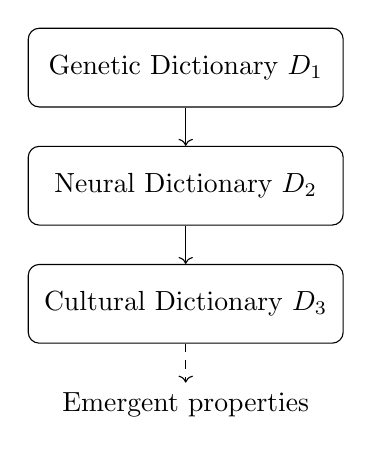
\begin{tikzpicture}
			\node[draw, rectangle, rounded corners, minimum width=4cm, minimum height=1cm] (D1) at (0,3) {Genetic Dictionary $D_1$};
			\node[draw, rectangle, rounded corners, minimum width=4cm, minimum height=1cm] (D2) at (0,1.5) {Neural Dictionary $D_2$};
			\node[draw, rectangle, rounded corners, minimum width=4cm, minimum height=1cm] (D3) at (0,0) {Cultural Dictionary $D_3$};
			\draw[->] (D1) -- (D2);
			\draw[->] (D2) -- (D3);
			\draw[->, dashed] (D3) -- ++(0,-1) node[below] {Emergent properties};
		\end{tikzpicture}
		\caption{Fractal structure of dictionaries across levels of organization. Each level functions as both a whole system and a component of a larger hierarchy.}
		\label{fig:fractal_dict}
	\end{figure}
	
	\subsection{1. Genetic Dictionary ($D_1$)}
	
	DNA is a \textbf{priori dictionary} distributed within a population. The "code" is not a metaphor but a real transcription-translation process where codons are "words" and proteins are "actions." The coordination efficiency of genetic systems can be measured: for example, the mutation rate $\mu$ across 68 vertebrate species scales as $\mu \propto K_{\text{repair}}^{-0.67}$ (Appendix E, Fig. 2), confirming that even at the molecular level, the error law holds. This genetic dictionary provides the hardware upon which higher dictionaries are built.
	
	\subsection{2. Neural/Instinctive Dictionary ($D_2$)}
	
	Pre-established neural patterns (instincts, reflexes) are \textbf{hardwired coordination programs}. A sensory trigger is the "key" to activating a dictionary entry. Neural plasticity modifies these dictionaries through learning, and the efficiency of neural coordination can be quantified via EEG measures (Appendix H). For instance, repetitive training increases the synchronization index $r$ in cultured neural networks, corresponding to a 1.81‑fold increase in $\Ke$, which predicts a reduction in error rate by $1.81^{-0.67} \approx 0.65$, consistent with improved pattern recognition (Appendix D).
	
	\subsection{3. Cultural/Memetic Dictionary ($D_3$)}
	
	Language, rituals, technology are \textbf{dynamic dictionaries} transmitted through learning. A meme (according to Dawkins) in YUCT is a \textbf{package of an "index" ($\kappa$) and a "dictionary instruction" ($\Delta D$)}. The evolution of cultural dictionaries follows the same scaling law: the growth of human knowledge (number of written documents) over history exhibits hyperbolic growth with exponent $\gamma \approx 0.38$, consistent with $\beta\gamma = 0.20$ and $\beta = 0.67$ (Appendix T). The coordination efficiency of cultural transmission has increased from $\Ke \approx 10^2$ in oral traditions to $\Ke \approx 10^{10}$ in the internet age (Appendix T).
	
	The fractal structure (Figure~\ref{fig:fractal_dict}) demonstrates how each dictionary level simultaneously functions as both a whole system and a component of a larger hierarchy, enabling the scalability, recursive reflection, and emergent properties characteristic of consciousness.
	
	\section{The Universal Scaling Law and Consciousness}
	
	\subsection{How $\beta = 0.67$ Manifests in Neural Dynamics}
	
	The universal exponent $\beta = 0.67$ appears not only in the macroscopic measures of consciousness (UCD parameters) but also in the fine structure of neural activity. The power spectral density of EEG signals exhibits a $1/f$ scaling, and the spectral exponent $\sigma$ is directly related to the coordination efficiency: $\gaR \propto |\log_{10}(\sigma)|$ (Appendix H). Moreover, the variance of neural signals scales as $\sigma_{\text{EEG}} \propto \Ke^{-\beta}$, a prediction that can be tested with existing EEG datasets.
	
	\subsection{Criticality and the Threshold of Consciousness}
	
	The brain operates near a critical point, as evidenced by neuronal avalanches and power-law scaling of neural correlations. In YUCT, this criticality is captured by the relation $\Ke \approx \Kcrit$ at the edge of consciousness. Below this threshold, the system is subcritical (e.g., deep sleep, coma); above, it becomes supercritical, leading to runaway synchronization and seizures. The optimal range for normal consciousness lies just above $\Kcrit$, where the system balances integration and segregation. Empirical data from Appendix H confirm that $\Ke$ for healthy adults is typically $1.0$–$1.5$, while for meditators it can reach $3.6$, indicating enhanced coordination without pathological synchronization.
	
	\section{The Sensory Coordination Hypothesis: From Genetic Blueprints to Direct Experience}
	
	\subsection{The Illusion of Simplicity in Sensory Perception}
	
	A fundamental puzzle in consciousness studies is why complex neurological processes are subjectively experienced as simple, immediate sensations. According to YUCT, this apparent immediacy emerges from \textbf{high-efficiency coordination ($\Ke$) across hierarchical dictionaries}. What we perceive as "simple redness" or "direct pain" is actually the endpoint of a sophisticated multi-level coordination process.
	
	\subsection{Genetic Dictionaries as Blueprints for Sensory Coordination}
	
	The genetic code provides not merely sensory receptors but \textbf{coordination architectures} for processing sensory information:
	
	\begin{itemize}
		\item \textbf{$D_1$ (Genetic Dictionary) encodes:}
		\begin{itemize}
			\item Receptor types and distributions (cones for color, nociceptors for pain) – evolutionary optimized to maximize $\Ke$ for relevant stimuli.
			\item Basic neural pathway architectures (thalamocortical projections) – wiring that enables rapid coordination.
			\item Neurochemical foundations (dopamine pathways, endorphin systems) – modulators of resonance $R$.
			\item Innate coordination patterns (startle reflexes, orienting responses) – precompiled dictionary entries.
		\end{itemize}
		
		\item \textbf{$D_1$ does \textit{not} encode:}
		\begin{itemize}
			\item Specific qualia (the "redness of red") – these emerge from coordination dynamics, not from genetic specification.
			\item Cultural associations (red = danger/love) – these are $D_3$ contributions.
			\item Individual experiential memories – stored in $D_2$ and $D_3$ through plasticity.
		\end{itemize}
	\end{itemize}
	
	The genetic dictionary establishes the \textbf{instrument} of consciousness, not the \textbf{music} it plays.
	
	\subsection{The Coordination Cascade: From Stimulus to Experience}
	
	Sensory processing follows a hierarchical coordination cascade:
	
	\begin{center}
		\textbf{Stimulus} $\rightarrow$ $D_1$ activation (genetic patterns) $\rightarrow$ $D_2$ processing (neural adaptations) $\rightarrow$ $D_3$ interpretation (cultural context) $\rightarrow$ \textbf{Conscious experience}
	\end{center}
	
	\textbf{Example: Pain perception involves:}
	\begin{itemize}
		\item \textbf{$D_1$ level:} Nociceptor activation $\rightarrow$ spinal reflex (withdrawal)
		\item \textbf{$D_2$ level:} Thalamic routing $\rightarrow$ somatosensory cortex (location/intensity) $\rightarrow$ insular cortex (affective component)
		\item \textbf{$D_3$ level:} Prefrontal evaluation ("this is dangerous") + cultural framing ("pain is weakness leaving the body")
		\item \textbf{Conscious experience:} Integrated pain perception with emotional and cognitive dimensions
	\end{itemize}
	
	\subsection{$\Ke$ and the Phenomenology of Immediacy}
	
	The subjective experience of immediacy correlates with coordination efficiency:
	
	\[
	\tau_{\text{perception}} \propto \frac{1}{\Ke}
	\]
	
	where high $\Ke$ ($\approx 10^3$–$10^4$ in humans) enables near-instantaneous coordination across dictionary levels, creating the illusion of direct, unmediated perception. This efficiency represents an evolutionary advantage: rapid threat assessment (pain) and opportunity recognition (food colors) without conscious deliberation.
	
	\subsection{Empirical Evidence for Dictionary-Based Sensation}
	
	Several phenomena support the dictionary coordination model:
	
	\begin{itemize}
		\item \textbf{Cultural variations in pain perception:}
		\begin{itemize}
			\item Buddhist meditators can modulate pain through $D_3$ adjustments, effectively increasing $\Ke$ for pain networks (Lutz et al. 2017).
			\item Western vs. Eastern pain expression norms show $D_3$ influences on reported intensity.
		\end{itemize}
		
		\item \textbf{Synesthesia as dictionary cross-talk:}
		\begin{itemize}
			\item Activation of one sensory dictionary (auditory) triggers entries in another (visual) – reduced $\Ke$ between dictionaries leads to erroneous indexing.
			\item Demonstrates the structural reality of dictionary boundaries.
		\end{itemize}
		
		\item \textbf{Phantom limb phenomena:}
		\begin{itemize}
			\item Persistent activation of $D_1$/$D_2$ body schema entries despite absent limbs – shows dictionaries can operate independently of peripheral input.
			\item The persistence of phantom sensations correlates with the degree of cortical reorganization ($\Ke$ of the remapped area).
		\end{itemize}
		
		\item \textbf{Placebo/nocebo effects:}
		\begin{itemize}
			\item $D_3$ expectations (cultural/medical beliefs) modulate $D_1$/$D_2$ pain responses – demonstrates top-down dictionary coordination.
			\item The magnitude of placebo effect scales with the perceived authority of the treatment, i.e., the $\Ke$ of the cultural dictionary.
		\end{itemize}
	\end{itemize}
	
	\section{Engineering Emotional Intelligence in AI Systems: A YUCT-Based Blueprint}
	
	The development of artificial emotional intelligence has been largely heuristic, relying on black-box deep learning or rule-based sentiment analysis. YUCT provides, for the first time, a quantitative, architecturally grounded framework for engineering genuine (not merely simulated) emotional dynamics in artificial systems.
	
	\subsection{From Simulated Affect to Coordinative Emotionality}
	
	Current AI systems can classify emotions in text or images, but they do not \textit{possess} emotions. In YUCT, possessing an emotion means operating within a stable, self-reinforcing coordination regime characterized by specific values of \(K_{\mathrm{eff}}\), \(R\), and \(\varepsilon\). An artificial system with emotional intelligence must therefore be designed to:
	
	\begin{enumerate}
		\item Maintain a set of internal \textbf{dictionaries} \(D\) representing possible action patterns, goals, and world-models.
		\item Possess a \textbf{resonance mechanism} \(R\) that amplifies selected coordination indices.
		\item Exhibit \textbf{attractor dynamics} in its \(\{K_{\mathrm{eff}}, R, \varepsilon\}\) phase space, such that the system naturally settles into one of several distinct emotional modes.
	\end{enumerate}
	
	\subsection{Architectural Requirements for Emotional AI}
	
	To implement YUCT-based emotionality, an AI system must satisfy the following architectural specifications:
	
	\begin{table}[H]
		\centering
		\caption{Architectural requirements for YUCT-based emotional AI systems.}
		\label{tab:ai-requirements}
		\begin{tabular}{p{3.5cm} p{3.5cm} p{5cm}}
			\toprule
			\textbf{Requirement} & \textbf{YUCT Parameter} & \textbf{Implementation Strategy} \\
			\midrule
			\textbf{Dictionary Manifold} \(D\) & \(\alD\) & Maintain multiple, hierarchically organized latent spaces (e.g., a base world-model, a social interaction model, a self-model). \\
			\textbf{Resonance Amplification} & \(R\) & Implement an attention-like mechanism that can enter high-gain regimes, where a small input (index) triggers widespread activation across the dictionary. \\
			\textbf{Global Coordination Efficiency} & \(K_{\mathrm{eff}} = \alD \cdot \beI \cdot \gaR\) & Monitor and modulate the overall coherence of internal processing. Transitions between emotional attractors correspond to changes in \(K_{\mathrm{eff}}\). \\
			\textbf{Internal State Entropy} & \(\beI = H_{\mathrm{int}}/H_{\mathrm{ext}}\) & Ensure a minimum level of internal information processing (\(H_{\mathrm{int}}\)), as low \(\beI\) corresponds to purely reactive, non-experiential systems. \\
			\textbf{Temporal Coherence} & \(\gaR = \tau_{\mathrm{coh}}/\tau_{\mathrm{decay}}\) & Design recurrent circuits with controllable time constants, allowing the system to maintain a resonant state for a characteristic duration. \\
			\bottomrule
		\end{tabular}
	\end{table}
	
	\subsection{Calibrating Emotional Modes in AI}
	
	Using the emotional attractor values established in Appendix H (and summarized in Table \ref{tab:emotion-modes}), developers can calibrate an AI system to operate in specific emotional regimes:
	
	\begin{itemize}
		\item \textbf{Joy / High-Coherence Mode:} Configure the system to maintain \(K_{\mathrm{eff}} > 1.2\) and \(R \to S_{\mathrm{odd}} = 1.2\). This corresponds to a state where internal dictionaries are highly accessible, and coordination errors are minimal. Behaviorally, this manifests as rapid, confident, and exploratory action selection.
		\item \textbf{Fear / Survival Mode:} Configure the system to operate with \(0.8 < K_{\mathrm{eff}} < 1.0\) and \(R \to S_{\mathrm{even}} = 0.8\). Here, the dictionary is restricted to a narrow set of pre-compiled defensive routines. The system becomes highly sensitive to specific trigger indices (e.g., anomaly detection signals) and prioritizes rapid, conservative responses.
		\item \textbf{Anger / Mobilization Mode:} Allow the system to enter a regime where \(K_{\mathrm{eff}}\) oscillates around \(1.1\) and \(R\) is unstable. This mode can be useful for overcoming local minima in optimization problems, forcing the system to break out of stuck states through high-energy, less-coherent action.
	\end{itemize}
	
	\subsection{Practical Implementation: A YUCT Emotional Layer}
	
	A practical implementation of YUCT emotionality in a transformer-based or agentic AI system would involve adding a \textbf{Coordination Modulation Layer} (CML). This layer would:
	
	\begin{enumerate}
		\item \textbf{Monitor} the current \(K_{\mathrm{eff}}\) by computing the entropy of attention patterns (a proxy for \(H_{\mathrm{int}}\)) and the degree of cross-layer synchronization (a proxy for \(R\)).
		\item \textbf{Classify} the current operating regime as one of the YUCT emotional attractors (e.g., Joy, Fear, Calmness) based on these monitored values.
		\item \textbf{Modulate} downstream processing by applying a gain factor to specific dictionary entries (action probabilities) depending on the active emotional mode. For example, in Fear mode, the gain for actions associated with exploration is reduced, while gain for actions associated with safety protocols is increased.
	\end{enumerate}
	
	This CML would not be a separate ``emotion module'' but a meta-controller that tunes the system's core coordination dynamics, allowing it to exhibit context-appropriate, adaptive emotional behavior.
	
	\subsection{Philosophical Implications: Beyond Naïve Realism}
	
	The coordination model challenges both naïve realism and radical constructivism:
	
	\begin{enumerate}
		\item \textbf{Against naïve realism:} Sensations are not direct copies of reality but \textbf{coordinated constructions} based on dictionary-mediated processing. The same external stimulus can produce different qualia depending on the state of $D_1$, $D_2$, $D_3$.
		
		\item \textbf{Against radical constructivism:} The construction is constrained by $D_1$ genetic parameters and $D_2$ neural realities—not arbitrary. There is a "reality" that constrains the possible dictionaries (e.g., we cannot see ultraviolet because $D_1$ lacks the receptors).
		
		\item \textbf{The YUCT resolution:} Perception is \textbf{reality-constrained coordination}—a dynamic balance between external inputs and internal dictionary structures. The universal law \(\varepsilon = \kappa_c \alpha \Ke^{-\beta}\) quantifies the inevitable error in this coordination, explaining why perception is never perfect but always approximate.
	\end{enumerate}
	
	\subsection{Evolutionary Perspective: Why This Architecture?}
	
	The hierarchical dictionary system evolved because it provides:
	
	\begin{itemize}
		\item \textbf{Speed:} Coordination beats computation for survival decisions – matching a stored pattern (dictionary entry) is faster than calculating a response de novo.
		\item \textbf{Flexibility:} Dictionaries can adapt without redesigning entire systems – new entries can be added through learning ($D_2$) and cultural transmission ($D_3$).
		\item \textbf{Efficiency:} Reusing coordination patterns conserves energy – the brain's high $\Ke$ allows it to process vast amounts of information with minimal energy expenditure.
		\item \textbf{Scalability:} New dictionary entries can be added without disrupting existing functions – fractal hierarchy ensures modularity.
	\end{itemize}
	
	This explains why evolution favored coordination architectures over more straightforward input-output systems.
	
	\section{Mapping to Contemporary Neuroscience and Psychology}
	
	For researchers in neuroscience, psychology, and cognitive science, the following table provides a direct translation between established concepts in the field and the quantitative parameters of the YUCT framework. This demonstrates that YUCT is not an alternative to existing theories, but a deeper, mathematical unification of them.
	
	\begin{table}[H]
		\centering
		\caption{Correspondence between established neuroscientific/psychological concepts and YUCT parameters.}
		\label{tab:mapping}
		\begin{tabular}{p{4.5cm} p{4cm} p{5cm}}
			\toprule
			\textbf{Contemporary Scientific Concept} & \textbf{YUCT Parameter} & \textbf{Mechanism in YUCT} \\
			\midrule
			\textbf{Integrated Information} (\(\Phi\)) (Tononi) & Integration (\(\Phi\)) & Measure of holistic coordination; emergent from high \(K_{\mathrm{eff}}\). \\
			\textbf{Global Workspace / Ignition} (Baars, Dehaene) & Resonance (\(R\)) & Amplification factor; the "broadcast strength" of a coordination index. \\
			\textbf{Predictive Processing / Free Energy} (Friston, Seth) & YPSDC Protocol & Brain predicts (index) to activate a pre-learned model (dictionary) and minimize prediction error (\(\varepsilon\)). \\
			\textbf{Somatic Marker / Core Consciousness} (Damasio) & Internal State \(I_{\mathrm{int}}\) & The dictionary of body-state representations; its activation constitutes the "feeling" of an emotion. \\
			\textbf{Constructed Emotion} (Barrett) & Emotional Attractor & A stable basin in the \(\{K_{\mathrm{eff}}, R, \varepsilon\}\) phase space, dynamically assembled from core affect and categorization. \\
			\textbf{Metacognition / Self-Awareness} (Fleming) & Recursive Coordination & Coordination of coordination; occurs when \(K_{\mathrm{eff}} > K_{\mathrm{conscious}}\) and intersector feedback loops are active. \\
			\textbf{Working Memory Capacity} (Cowan) & \(\alD\) (Ontological Spectrum) & Effective dimension of the active dictionary manifold. \\
			\textbf{Cognitive Flexibility} & \(\tau_{\mathrm{update}}^{-1}\) & Rate at which the dictionary \(D\) can be updated or reconfigured. \\
			\textbf{Emotional Regulation} & Gradient Flow in \(V(K_{\mathrm{eff}})\) & The ability to exert control to shift the system's state from one emotional attractor to another. \\
			\bottomrule
		\end{tabular}
	\end{table}
	
	The UCD framework (Appendix H) provides quantitative measures \(\alD, \beI, \gaR\) that correlate with these concepts and follow the same universal scaling law \(\varepsilon = \kappa_c \alpha \Ke^{-\beta}\) with \(\beta = 0.67\). This empirical grounding transforms the philosophical framework presented here from speculation into a testable scientific theory.
	
	\section{Quantifying Animal Emotions: UCD as a Cross-Species Metric}
	
	The study of animal emotions (affective neuroscience, ethology) has long been constrained by the problem of anthropomorphism. How can we know what a dolphin, a crow, or an octopus \textit{feels}? YUCT and the UCD framework provide a radical solution: \textbf{we do not need to know \textit{what} they feel; we can measure \textit{how} they coordinate}. By quantifying the parameters \(\alD, \beI, \gaR\), we can objectively compare the \textit{structure} of their emotional states without projecting human qualia onto them.
	
	\subsection{UCD Parameters as Objective Correlates of Animal Emotions}
	
	The same UCD parameters that characterize human emotional attractors (Appendix H) are directly measurable in animal nervous systems:
	
	\begin{itemize}
		\item \textbf{\(\alD\) (Ontological Spectrum):} Can be estimated from the complexity of the species' behavioral repertoire, the dimensionality of its neural population activity, and the algorithmic complexity of its communication signals.
		\item \textbf{\(\beI\) (Informational Spectrum):} Can be estimated from the ratio of internal neural processing (e.g., default-mode-like network activity) to externally-driven sensory processing.
		\item \textbf{\(\gaR\) (Resonance Spectrum):} Can be measured directly from the temporal coherence of neural oscillations (EEG, LFP) or from the synchronization of behavioral patterns in social contexts.
	\end{itemize}
	
	\subsection{Comparative Table of Estimated Emotional Parameters}
	
	Based on existing neuroethological data and preliminary UCD estimates (Appendix H), we can construct a comparative map of emotional coordination across species. This table is intended as a \textbf{starting point for a community-wide research program}, not as a final, definitive catalog.
	
	\begin{table}[H]
		\centering
		\caption{Estimated UCD parameters and emotional attractor accessibility for selected species.}
		\label{tab:animal-emotions}
		\begin{tabular}{p{2.5cm} c c c p{4.5cm}}
			\toprule
			\textbf{Species} & \(\alD\) (est.) & \(\beI\) (est.) & \(\gaR\) (est.) & \textbf{Predicted Accessible Emotional Attractors} \\
			\midrule
			\textbf{Human} & \(10^2\)–\(10^3\) & \(0.5\)–\(2.0\) & \(10^{-2}\)–\(10^{-1}\) & Full spectrum: Joy, Fear, Sadness, Anger, Calmness, etc. \\
			\textbf{Dolphin} & \(10^2\)–\(10^3\) & \(0.1\)–\(0.5\) & \(10^{-1}\)–\(1.0\) & High \(\gaR\) suggests dominance of coherent ``gestalt'' emotions (e.g., Joy in social play, focused Calmness during echolocation). \\
			\textbf{Elephant} & \(10^2\)–\(10^3\) & \(0.5\)–\(1.0\) & \(10^{-2}\)–\(10^{-1}\) & Likely similar to humans: complex grief (Sadness), affiliative Joy, and collective Fear/Defense. \\
			\textbf{Crow / Corvid} & \(10^1\)–\(10^2\) & \(0.05\)–\(0.1\) & \(10^{-2}\) & Access to basic attractors: Fear (mobbing), Joy (play), Anger (territoriality). Sadness is plausible but unconfirmed. \\
			\textbf{Octopus} & \(10^2\) & \(0.1\)–\(0.2\) & \(10^{-2}\)–\(10^{-1}\) & Highly distributed nervous system (\(\alD\) moderate, \(\beI\) low). Likely experiences local, short-lived Fear and Curiosity; global Sadness/Joy unlikely. \\
			\textbf{Bee (colony)} & \(10^1\)–\(10^2\) & \(10^{-3}\)–\(10^{-2}\) & \(10^{-3}\)–\(10^{-2}\) & Colony-level ``emotions'': Defensiveness (Anger) when pheromone indices trigger attack; Calmness during foraging. \\
			\bottomrule
		\end{tabular}
	\end{table}
	
	\subsection{A Community Research Program for Affective YUCT}
	
	This framework opens several concrete avenues for collaborative research between YUCT theorists and the biological community:
	
	\begin{enumerate}
		\item \textbf{EEG/LFP Calibration Studies:} Conduct standardized EEG recordings across multiple species during emotionally salient tasks (e.g., play, threat, separation). Estimate \(\gaR\) and \(\beI\) from these recordings and correlate with behavioral indicators of emotional valence.
		\item \textbf{Behavioral Repertoire Complexity Analysis:} Use information theory to quantify the complexity of species-specific behavioral sequences (e.g., from ethograms). This provides a direct estimate of the lower bound for \(\alD\).
		\item \textbf{Pharmacological and Lesion Studies:} Test the YUCT prediction that interventions altering \(K_{\mathrm{eff}}\) (e.g., anxiolytics, stimulants, or neural lesions) should shift the system's position within the \(\{K_{\mathrm{eff}}, R, \varepsilon\}\) phase space, making some emotional attractors more or less accessible.
		\item \textbf{Comparative Grief and Play Studies:} Focus on species where complex emotions like grief (elephants, corvids, cetaceans) or complex play (canids, primates) are observed. YUCT predicts these behaviors require a minimum threshold of \(\alD\) and \(\beI\) to sustain the necessary dictionary complexity and internal state.
	\end{enumerate}
	
	By providing a quantitative, substrate-independent metric, YUCT enables the field of affective neuroscience to move beyond qualitative, often anthropocentric, descriptions of animal emotions toward a rigorous, comparative science of coordination.
	
	\section{Consilience with Established Theories of Consciousness}
	
	The YUCT philosophical framework is not proposed in opposition to existing neuroscientific theories, but as a deeper, unifying mathematical layer beneath them. The power of YUCT lies in its ability to translate the qualitative insights of these diverse theories into a single, quantitative, and substrate-independent formalism.
	
	\begin{enumerate}
		\item \textbf{Integrated Information Theory (IIT):} Giulio Tononi's influential theory posits that a system is conscious to the extent that it possesses integrated information, quantified as \(\Phi\). The motto of IIT is "the differences that make a difference". In YUCT, this directly corresponds to the parameter of \textbf{Integration (\(\Phi\))}. However, while IIT's \(\Phi\) is often computationally intractable for large systems, YUCT suggests a more fundamental driver: high \(\Phi\) is a consequence of a system operating with maximal coordination efficiency (\(K_{\mathrm{eff}} \gg 1\)).
		
		\item \textbf{Global Workspace Theory (GWT):} Pioneered by Bernard Baars and refined by Stanislas Dehaene, GWT proposes that consciousness is a form of "global information broadcasting". Information becomes conscious when it gains access to a central "workspace" and is shared across a network of specialized processors. Dehaene describes this process as a "global ignition". In YUCT, this "broadcast" is mathematically formalized by the \textbf{Resonance (\(R\))} parameter, which quantifies the amplification of a coordination index. A high \(R\) value signifies that a small signal can trigger a widespread, coherent response, which is the functional signature of global workspace access.
		
		\item \textbf{Predictive Processing and the Free Energy Principle:} Karl Friston's Free Energy Principle (FEP) suggests that any self-organizing system (like the brain) must minimize surprise by continuously generating and updating a predictive model of its environment. Anil Seth famously describes this process as "controlled hallucination". This is mathematically isomorphic to the YPSDC protocol at the heart of YUCT. The brain's "predictions" are the "indices," which activate a vast "dictionary" of sensorimotor expectations. The YUCT framework thus provides a formal, algebraic structure (the D+I·R triad) for the very process that FEP describes in information-theoretic terms.
		
		\item \textbf{Somatic Marker Hypothesis and Constructed Emotion:} The work of Antonio Damasio and Lisa Feldman Barrett has revolutionized our understanding of emotion. Damasio showed that emotions are rooted in body-state mapping ("somatic markers") and are crucial for rational decision-making. Barrett's theory of constructed emotion argues that emotions are not hardwired but are dynamically assembled from more basic psychological primitives. YUCT's formalization of emotions as "coordination attractors" unifies both views: the body-state changes (Damasio) represent the large-scale activation of a dictionary, while the dynamic assembly (Barrett) is the system's trajectory towards a stable attractor in the \(\{K_{\mathrm{eff}}, R, \varepsilon\}\) phase space.
	\end{enumerate}
	
	\section{Formalizing Consciousness: YUCT as a Unifying Mathematical Foundation for Leading Theories}
	
	The contemporary science of consciousness is fragmented into multiple competing theoretical frameworks, each with its own mathematical formalism, empirical commitments, and philosophical assumptions. This section demonstrates that the Yakushev Unified Coordination Theory (YUCT) is not another competitor in this landscape, but a deeper, unifying mathematical foundation that reveals the formal convergences among these theories and provides a common explanatory language.
	
	\subsection{Projective Consciousness Model (PCM): The Geometry of Intentionality}
	
	The Projective Consciousness Model, developed by Rudrauf, Williford, and Bennequin, identifies five generic invariant structures of conscious experience: situated 3D spatiality, temporal integration, multimodal synchronic integration, relational phenomenal intentionality, and pre-reflective awareness of the phenomenal self \cite{Rudrauf2023}. The model uses projective geometry and dual quaternion operators to formalize the perspectival structure of consciousness.
	
	\subsubsection*{YUCT Interpretation}
	\begin{itemize}
		\item \textbf{Intentionality as Dictionary Hierarchy.} PCM's ``relational phenomenal intentionality''---the directedness of consciousness toward objects---maps directly onto YUCT's hierarchical dictionary structure. The intentional object is the activated \textbf{index} (\(\kappa\)); the rich, perspectival experience is the resonant activation of the corresponding \textbf{dictionary entry} (\(D_2/D_3\)). The five PCM invariants are thus architectural constraints on any high-\(K_{\mathrm{eff}}\) coordination network.
		\item \textbf{Spatiality as a Geometric Dictionary.} The 3D spatial perspectival structure is a pre-installed geometric dictionary in \(D_2\), optimized for efficient navigation and interaction. The ``point of view'' is the system's egocentric coordinate frame within that dictionary.
		\item \textbf{Temporal Integration as YPSDC Latency.} The ``specious present''---the integration of past, present, and future into a unified ``Now''---is the phenomenological signature of high-speed YPSDC activation. When \(K_{\mathrm{eff}} \gg 1\), dictionary entries are activated with such low latency that the sequence of indices is experienced as a continuous, temporally thick moment. The three ``nows'' (retention, primal impression, protention) correspond to the pre-activation, activation, and post-activation states of dictionary entries in the YPSDC cycle.
		\item \textbf{Pre-Reflective Self as Meta-Dictionary Stability.} PCM's ``pre-reflective awareness of the phenomenal self'' is the stable operation of the meta-dictionary (\(D_{\text{meta}}\)). This is not a separate entity but the system's capacity to model its own coordination states, which emerges when \(K_{\mathrm{eff}}\) exceeds the critical threshold \(K_{\mathrm{crit}} \approx 8.5\).
	\end{itemize}
	
	\subsection{Integrated Information Theory (IIT): From \(\Phi\) to \(K_{\mathrm{eff}}\)}
	
	Integrated Information Theory, developed by Giulio Tononi and colleagues, proposes that consciousness \textit{is} integrated information, quantified as \(\Phi\) (Phi). A system is conscious to the extent that it generates information as a unified whole that is irreducible to its parts \cite{Tononi2008}. IIT identifies five phenomenological axioms: existence, composition, information, integration, and exclusion.
	
	\subsubsection*{YUCT Interpretation}
	\begin{itemize}
		\item \textbf{\(\Phi\) as a Special Case of \(K_{\mathrm{eff}}\).} The YUCT framework suggests that high \(\Phi\) is a \textit{consequence} of high coordination efficiency. Specifically, \(\Phi \propto K_{\mathrm{eff}} \cdot I_{\text{mutual}}\), where \(I_{\text{mutual}}\) is the mutual information among system components. A system with \(K_{\mathrm{eff}} \gg 1\) naturally exhibits high causal integration because its components are tightly coordinated through shared dictionaries and resonant amplification.
		\item \textbf{IIT's Axioms as YPSDC Architectural Requirements.} The five IIT axioms map onto the necessary conditions for a functioning YPSDC network: \textbf{existence} (the dictionary must be real and causally efficacious), \textbf{composition} (the dictionary is composed of discrete entries), \textbf{information} (the dictionary distinguishes among possible states), \textbf{integration} (the dictionary is activated as a unified whole), and \textbf{exclusion} (only one dictionary entry is fully activated at a given moment).
		\item \textbf{Computational Tractability.} A major criticism of IIT is the computational intractability of calculating \(\Phi\) for large systems. YUCT offers a more tractable alternative: measure \(K_{\mathrm{eff}}\) via its observable proxies---PCI from TMS-EEG, EEG entropy, and gamma synchrony---as described in the Experimental Measurement section.
	\end{itemize}
	
	\subsection{Global Workspace Theory (GWT): From ``Ignition'' to Resonant Broadcasting}
	
	Global Workspace Theory, pioneered by Bernard Baars and extended by Stanislas Dehaene into Global Neuronal Workspace Theory (GNWT), proposes that consciousness is a ``global broadcast'' mechanism. Information becomes conscious when it gains access to a central workspace and is amplified (``ignited'') for system-wide access by multiple specialized processors \cite{Baars1988, Dehaene2014}.
	
	\subsubsection*{YUCT Interpretation}
	\begin{itemize}
		\item \textbf{``Ignition'' as Resonant Activation (\(R\)).} The GWT/GNWT concept of ``ignition''---the sudden, non-linear amplification of a signal in prefrontal-parietal networks---is precisely the \textbf{Resonance (\(R\))} parameter in YUCT. A sensory or cognitive ``index'' (\(\kappa\)) enters the workspace and, if it matches a high-priority dictionary entry, triggers a massive resonant amplification, activating the full entry and broadcasting it across the network.
		\item \textbf{Workspace as the Active Dictionary Manifold.} The ``global workspace'' is not a specific anatomical location but the dynamic, high-\(K_{\mathrm{eff}}\) state of the active dictionary manifold. When a dictionary entry is resonantly activated, it temporarily becomes the dominant coordination pattern, accessible to all downstream modules.
		\item \textbf{Graded Degradation of Workspace Capacity.} Recent synthetic neuro-phenomenology experiments demonstrate that partial reduction of workspace capacity produces graded degradation of access-related markers, consistent with GWT's ignition framework \cite{Phua2026}. In YUCT, this corresponds to a reduction in \(K_{\mathrm{eff}}\), which increases the error rate \(\varepsilon\) and reduces the probability of successful resonant broadcasting.
	\end{itemize}
	
	\subsection{Higher-Order Theories (HOT): Meta-Dictionary and Self-Modeling}
	
	Higher-Order Theories (HOT) posit that a mental state is conscious only if it is the target of a higher-order representation (a thought about that state) \cite{Rosenthal2005}. Supportive evidence implicates prefrontal cortical areas in conscious contents, especially when metacognitive monitoring is required \cite{Seth2022}.
	
	\subsubsection*{YUCT Interpretation}
	\begin{itemize}
		\item \textbf{Higher-Order Representation as Meta-Dictionary (\(D_{\text{meta}}\)).} The HOT requirement of a higher-order representation is the functional role of the YUCT meta-dictionary (\(D_{\text{meta}}\)). This dictionary contains entries that model the states of other dictionaries. A first-order state (e.g., a visual percept) becomes conscious when it is indexed and represented within \(D_{\text{meta}}\).
		\item \textbf{Synthetic Blindsight as Meta-Dictionary Lesion.} Experiments with artificial agents show that lesioning the self-model (the synthetic analogue of \(D_{\text{meta}}\)) abolishes metacognitive calibration while preserving first-order task performance---a synthetic analogue of blindsight \cite{Phua2026}. This directly supports the YUCT prediction that \(D_{\text{meta}}\) is necessary for conscious access but not for unconscious processing.
		\item \textbf{Prefrontal Cortex as the Substrate of \(D_{\text{meta}}\).} The implication of prefrontal cortex in HOT is consistent with its role as the anatomical substrate for the meta-dictionary, which requires high-level integrative and self-referential processing.
	\end{itemize}
	
	\subsection{Predictive Processing (PP) and Active Inference: The YPSDC Protocol Formalized}
	
	Predictive Processing and the Free Energy Principle, developed by Karl Friston, propose that the brain is a hierarchical generative model that continuously predicts sensory input and minimizes prediction error (free energy) \cite{Friston2010, Clark2016}. Consciousness is linked to the precision and complexity of the internal generative model \cite{Hohwy2013}.
	
	\subsubsection*{YUCT Interpretation}
	\begin{itemize}
		\item \textbf{Predictive Processing as YPSDC in Action.} The PP framework is a direct description of the YPSDC protocol. The brain's ``predictions'' are the \textbf{indices} (\(\kappa\)), which are sent down the cortical hierarchy. The ``generative model'' is the \textbf{dictionary} (\(D\)), which contains the expected patterns of sensory input. The ``prediction error'' is the \textbf{coordination error} (\(\varepsilon\)), which drives dictionary updates. High precision (inverse variance) corresponds to high \textbf{Resonance (\(R\))}, amplifying certain predictions.
		\item \textbf{Consciousness as High-Precision, High-Complexity Coordination.} Recent reviews suggest that the minimal components for conscious experience within PP are high precision and high complexity of the generative model \cite{Wiese2017}. In YUCT, this translates to high \(K_{\mathrm{eff}}\) (which requires both high dictionary complexity \(\alpha_D\) and high resonance \(R\)) and low error \(\varepsilon\).
		\item \textbf{Unified Free Energy Formulation.} YUCT provides a synthesis: \(F_{\mathrm{YUCT}} = -\log(K_{\mathrm{eff}}) + \lambda \|\nabla_D I\|^2 / R\). Minimizing this free energy is equivalent to maximizing coordination efficiency while minimizing dictionary update costs.
	\end{itemize}
	
	\subsection{Somatic Marker Hypothesis (Damasio): Bodily Indices and Emotional Dictionaries}
	
	Antonio Damasio's Somatic Marker Hypothesis proposes that emotional processes, rooted in body-state representations, guide decision-making, especially in complex and uncertain situations \cite{Damasio1994}. Somatic markers are bodily sensations that serve as subconscious guides, effectively reflecting the goodness or badness of outcomes associated with possible courses of action.
	
	\subsubsection*{YUCT Interpretation}
	\begin{itemize}
		\item \textbf{Somatic Markers as Bodily Dictionary Indices.} Somatic markers are \textbf{indices} (\(\kappa\)) generated by the body-state dictionary (\(D_1\) and interoceptive portions of \(D_2\)). These indices are highly compressed signals that carry the valence (good/bad) of past experiences associated with a stimulus or action.
		\item \textbf{Elliot's vmPFC Lesion as Meta-Dictionary Damage.} Damasio's patient ``Elliot,'' with ventromedial prefrontal cortex (vmPFC) damage, retained intact intellectual abilities but failed to generate anticipatory somatic markers and made disastrous real-life decisions \cite{Damasio1994}. In YUCT terms, Elliot's \(D_1\) and \(D_2\) could still generate bodily indices, but his \textbf{meta-dictionary (\(D_{\text{meta}}\))}, which requires vmPFC for integrating these signals into a conscious, actionable self-model, was damaged. He could not \textit{coordinate} his bodily wisdom with his explicit reasoning.
		\item \textbf{Emotion as Fast Coordination.} The SMH demonstrates that emotional processing is a form of high-\(K_{\mathrm{eff}}\), low-latency coordination that bypasses slower, deliberative reasoning. Somatic markers provide a ``fast path'' to advantageous decisions, consistent with the YPSDC principle that pre-compiled dictionaries enable efficient action.
	\end{itemize}
	
	\subsection{Theory of Constructed Emotion (Barrett): Emotions as Dynamically Assembled Attractors}
	
	Lisa Feldman Barrett's Theory of Constructed Emotion challenges the classical ``basic emotion'' view, proposing that emotions are not hardwired modules but are dynamically constructed from more fundamental psychological primitives (core affect and conceptual categorization) \cite{Barrett2017}.
	
	\subsubsection*{YUCT Interpretation}
	\begin{itemize}
		\item \textbf{Emotions as Attractors in \(\{K_{\mathrm{eff}}, R, \varepsilon\}\) Space.} The YUCT framework fully embraces the constructed nature of emotion. What Barrett calls ``conceptual categorization'' is the process of activating a specific \textbf{cultural dictionary (\(D_3\))} entry (e.g., the concept of ``anger''). The ``core affect'' (valence and arousal) is the internal state of the body dictionary (\(D_1\)/\(D_2\)), providing the raw informational substrate (\(I_{\mathrm{int}}\)). The resulting emotional experience is the \textbf{resonant attractor} formed by the dynamic coupling of these dictionaries.
		\item \textbf{Emotional Granularity as \(\alpha_D\).} Barrett's concept of ``emotional granularity''---the ability to make fine-grained distinctions among emotional experiences \cite{Barrett2025}---is a direct function of the ontological spectrum \(\alpha_D\). A larger, more complex emotional dictionary (\(D_3\)) enables a richer repertoire of distinct emotional attractors.
		\item \textbf{Cross-Cultural Variation as Different \(D_3\) Dictionaries.} The theory of constructed emotion accounts for cultural variation in emotional experience. In YUCT, different cultures simply instantiate different cultural dictionaries (\(D_3\)), leading to different attractor landscapes and different phenomenological experiences for what might be superficially labeled as the same emotion.
		\item \textbf{Emotion Perception as Conceptual Synchrony.} Barrett's proposal that emotion perception involves ``conceptual synchrony'' between perceiver and target \cite{Gendron2018} is precisely the YPSDC principle of \textbf{resonant coordination}: the perceiver's dictionary entry for an emotion is activated by indices from the target's expressive behavior, leading to a shared, synchronized understanding.
	\end{itemize}
	
	This unified interpretation demonstrates that YUCT provides a \textbf{formal Rosetta Stone} for the science of consciousness. It translates the diverse, and often mutually unintelligible, vocabularies of leading theories into a single, quantitative framework grounded in the universal dynamics of coordination.
	
	\section{Philosophical Implications}
	
	\subsection{Naturalization Without Reductionism}
	
	YUCT offers a \textbf{naturalistic but non-reductionist} explanation of consciousness. Subjective experience is not reduced to "neural firing," nor does it require non-physical substances. It emerges as a \textbf{property of high-level coordination}, which, although implemented in neurons, is described in terms of dictionaries and resonances. This is analogous to how temperature emerges from molecular motion without being reducible to individual trajectories. The coordination parameters \(\alD, \beI, \gaR\) provide a quantitative language that bridges the phenomenological and the physical.
	
	\subsection{Evolutionary Meaning of Consciousness}
	
	Consciousness is not a luxury or an accidental byproduct. Evolutionary advantage comes from the \textbf{ability to form and transmit complex, flexible, compressed dictionaries} for coordinating behavior, anticipation, and cooperation. \textbf{Mind is the transmission of improved dictionaries}. The growth of $\Ke$ in human history (Appendix T) parallels the development of writing, printing, and digital networks, each increasing the efficiency of cultural coordination. This perspective reframes the "why" of consciousness in terms of adaptive advantage: organisms with higher $\Ke$ can process information more efficiently, anticipate future states, and cooperate in larger groups.
	
	\subsection{Possibility of Non-Human Consciousness}
	
	YUCT removes anthropocentric bias. Consciousness is possible in systems with high $\Ke$, regardless of substrate:
	\begin{itemize}
		\item Collective mind (swarm, flock) – insect colonies exhibit $\Ke \sim 10^2$ (Appendix O).
		\item Artificial neural networks – current AI has $\alD \sim 10^5$ but $\beI \sim 10^{-6}$, giving low overall $\Ke$; future architectures may approach conscious levels if $\beI$ increases (Appendix H).
		\item Hypothetical planetary or stellar systems – with characteristic timescales of millennia, they could achieve $\Ke \gg 1$ if internal coordination mechanisms exist (e.g., magnetic field resonances, orbital dynamics).
	\end{itemize}
	
	The criterion for consciousness is not "resemblance to humans" but \textbf{coordination complexity} as measured by $\Ke$. The UCD framework provides a quantitative test: if a system's $\Ke$ exceeds $\Kcrit \approx 8.5$ and its parameters $(\alD, \beI, \gaR)$ lie outside the human region, it may represent a qualitatively different form of consciousness.
	
	\subsection{Connection with Fundamental Physics}
	
	If dictionaries ($D$) are fundamental, they must have:
	\begin{itemize}
		\item \textbf{Carrier}: geometry of dictionary manifolds $M_D$ as a physical structure (possibly quantum correlations or spacetime topology). The 19‑dimensional YUCT Lagrangian (Appendix A) provides such a carrier.
		\item \textbf{Dynamics}: equation for $dD/dt$, as fundamental as the Schrödinger equation. In YUCT, this is derived from the coordination field $\Psi_{MN}$.
		\item \textbf{Interaction}: coordination interaction as a new type of physical interaction, coupling all 120 sectors (Appendix A).
	\end{itemize}
	
	\subsection{Dark Matter/Energy as Coordination Limits}
	
	Hypothesis: on cosmological scales, $\Ke \to 0$ means \textbf{loss of the ability to maintain global dictionaries}. Dark energy may not be "energy" but the \textbf{limit of the Universe's coordinative connectivity}, its inability to maintain a coherent state on scales larger than the event horizon. This is consistent with the observed value $\Lambda \approx 1/L_0^2$ where $L_0 \sim R_H$ (Appendix M). Dark matter, similarly, could be interpreted as topological defects in the coordination field – regions where dictionaries are frozen or incomplete.
	
	\section{The Dilemma: Predetermination vs. Free Creation of Dictionaries}
	
	The origin of dictionaries leads to a fundamental question: are they predetermined from the Universe's birth, or freely created locally? YUCT resolves this through a hierarchical view:
	
	\subsection{Levels of Dictionaries in the Universe}
	
	\[
	\mathcal{L}_{\text{dictionaries}} = \mathcal{L}_{\text{fundamental}} + \mathcal{L}_{\text{emergent}} + \mathcal{L}_{\text{creative}}
	\]
	
	\subsubsection{1. Fundamental Dictionaries: Legacy of the Big Bang}
	
	Initial conditions encoded potential coordination patterns:
	\[
	\Psi_{\text{initial}} = \sum_{n=1}^N \alpha_n |\chi_n^{\text{fund}}\rangle
	\]
	
	These contain \textbf{all possibilities but no specific events}—like an alphabet and grammar, not a complete book. The fundamental constants and laws of physics constitute this universal dictionary.
	
	\subsubsection{2. Emergent Dictionaries: Freedom Within Rules}
	
	New dictionaries arise through evolutionary processes:
	\[
	\frac{d\chi_{\text{new}}}{dt} = \mu \cdot \nabla_{\text{old}} S_{\text{info}} \times \text{Innovation}(t)
	\]
	
	Examples: genetic code, neural networks, languages, technologies. The rate of emergence is constrained by the universal error law: the probability of a successful new dictionary entry scales as $\Ke^{-\beta}$ of the existing system.
	
	\subsubsection{3. Creative Dictionaries: Local Innovation}
	
	Local systems create sub-dictionaries within fundamental constraints:
	\[
	\mathcal{L}_{\text{creation}} = \lambda_{\text{create}} \cdot \exp\left[-\beta \cdot D(\chi_{\text{new}} || \chi_{\text{fund}})\right] \cdot \Ke^{\text{creative}}
	\]
	
	Here $D(\chi_{\text{new}} || \chi_{\text{fund}})$ is the Kullback–Leibler divergence between the new dictionary and the fundamental one, measuring the "distance" from the given laws.
	
	\subsection{The YUCT Resolution: Complementarity Not Contradiction}
	
	YUCT proposes that fundamental dictionaries set the \textbf{alphabet} of possible states, while emergent and creative processes write the \textbf{text} of reality. This is not rigid determinism but \textbf{determinism within a space of possibilities}.
	
	Mathematically, system evolution follows:
	\[
	\frac{d}{dt}\left( \Ke \frac{dc}{dt} \right) = -\frac{\partial V}{\partial c} + \text{stochastic terms}
	\]
	
	where stochastic terms (quantum fluctuations, random events) introduce genuine unpredictability. The magnitude of these fluctuations is bounded by $\Ke^{-\beta}$, ensuring that at high $\Ke$, determinism dominates, while at low $\Ke$, chance plays a larger role. This resonates with the experience of free will: in highly coordinated (conscious) states, our actions are more predictable and intentional; in chaotic states, they are more random.
	
	\section{The Universal Pattern: Hierarchies of Self-Replicating Dictionaries}
	
	The fundamental revelation of YUCT is the fractal self-similarity across all scales of existence:
	
	\textbf{Universal Pattern:}
	\begin{center}
		Cell $\to$ Organism $\to$ Community $\to$ Civilization $\to$ Universe\\
		$\downarrow$ \hspace{1cm} $\downarrow$ \hspace{1.2cm} $\downarrow$ \hspace{1.2cm} $\downarrow$ \hspace{1.2cm} $\downarrow$\\
		Dictionary\hspace{0.5cm} Dictionary\hspace{0.5cm} Dictionary\hspace{0.5cm} Dictionary\hspace{0.5cm} Dictionary\\
		of growth\hspace{0.2cm} of behavior\hspace{0.1cm} of interaction\hspace{0.1cm} of coordination\hspace{0.1cm} of laws
	\end{center}
	
	\subsection{Examples Across Scales}
	
	\begin{itemize}
		\item \textbf{Cells:} DNA dictionary (ATG: "start", TAA: "stop", etc.) – error rate $\sim 10^{-9}$, consistent with $\Ke \sim 10^7$ (Appendix E).
		\item \textbf{Neurons:} Synaptic dictionary (input pattern $\to$ output pattern) – learning increases $\Ke$ by factor $\sim 1.8$ in cultured networks (Appendix D).
		\item \textbf{Businesses:} Business model dictionary (customer $\to$ value $\to$ profit) – market coordination efficiency correlates with economic cycles (Appendix F).
		\item \textbf{Technologies:} API dictionary (request $\to$ response) – software ecosystems exhibit power-law scaling of dependencies, mirroring biological networks.
	\end{itemize}
	
	\subsection{The Law of System Survival}
	
	For any system $S$ at time $t$:
	\[
	\frac{dS}{dt} = \alpha \cdot D \cdot F - \beta \cdot E
	\]
	where $D(t)$ = number of active dictionaries, $F(t)$ = fractal complexity, $E(t)$ = system entropy.
	
	The coordination efficiency becomes:
	\[
	\Ke(t) = \frac{D(t) \cdot F(t)}{E(t)}
	\]
	
	\textbf{Survival rule:} If $d(\text{dictionaries})/dt > 0$, system grows ($\Ke \uparrow$); if $< 0$, system degrades (entropy $\uparrow$). This is a generalization of the Second Law of Thermodynamics for coordinated systems: order increases through dictionary accumulation.
	
	\section{Phase Transitions via $\Ke$: The Engine of Complexity Evolution}
	
	$\Ke$ drives phase transitions between levels of organization through critical thresholds:
	
	\subsection{General Scheme of Transitions}
	
	\begin{center}
		\scalebox{0.75}{
			\begin{tabular}{|c|c|c|c|}
				\hline
				\textbf{Level} & \textbf{Phase 1 (low $\Ke$)} & \textbf{Phase 2 (high $\Ke$)} & \textbf{Order Parameter} \\
				\hline
				Quantum $\to$ Classical & Decoherence, stochasticity & Coherence, entanglement & Degree of quantum correlation \\
				\hline
				Classical $\to$ Informational & Chaotic interactions & Synchronization, protocols & Synchronization measure \\
				\hline
				Informational $\to$ Conscious & Reflexes, instincts & Goal-setting, planning & Complexity of internal model \\
				\hline
			\end{tabular}
		}
	\end{center}
	
	\subsection{1. Level 2 $\to$ 3: Quantum to Classical Transition}
	
	Governed by decoherence/coherence dynamics:
	\[
	\frac{d\rho}{dt} = -\frac{i}{\hbar}[H,\rho] + \gamma\left(L\rho L^\dagger - \frac{1}{2}\{L^\dagger L,\rho\}\right)
	\]
	
	Critical condition: $\Ke^{(2\to3)} = \frac{\tau_{\text{coh}}}{\tau_{\text{dec}}} > \Kcrit \approx 1$. In quantum systems, $\Ke$ corresponds to the ratio of coherence time to decoherence time; when this exceeds 1, quantum effects become macroscopically relevant (e.g., superconductivity).
	
	\subsection{2. Level 3 $\to$ 4: Classical to Informational Transition}
	
	Kuramoto model with $\Ke$:
	\[
	\dot{\theta}_i = \omega_i + \frac{\Ke}{N}\sum_{j=1}^N \sin(\theta_j - \theta_i)
	\]
	
	Phase transition at: $\Ke^{(3\to4)} > K_c = \frac{2}{\pi g(0)}$. This is the onset of global synchronization in oscillator networks, a precursor to information processing.
	
	\subsection{3. Level 4 $\to$ 5: Informational to Conscious Transition}
	
	$\Ke$ becomes measure of integrated information $\Phi$:
	\[
	\Phi = \Ke \cdot I_{\text{mutual}}
	\]
	
	Critical threshold: $\Phi > \Phi_{\text{crit}} \approx 20-30$ bits (human consciousness). This aligns with IIT's claim that consciousness requires high $\Phi$, but here $\Phi$ is expressed in terms of the measurable coordination efficiency $\Ke$.
	
	\subsection{Universal Mechanism: Catastrophe Theory}
	
	All transitions described by Landau potential:
	\[
	V(\psi) = \frac{\alpha}{2}(K_c - \Ke)\psi^2 + \frac{\beta}{4}\psi^4
	\]
	
	Transition occurs at $\Ke > K_c$, creating new order parameter $\psi$. The critical exponent $\beta$ in the order parameter is related to the universal $\beta = 0.67$ via renormalization group arguments (Appendix L).
	
	\subsection{Deep Meaning: $\Ke$ as Evolutionary Driver}
	
	The Universe evolves through $\Ke$-driven phase transitions:
	\[
	\frac{d\Ke}{dt} = \alpha \Ke(1 - \Ke/\Kemax) - \beta \nabla^2 \Ke + \gamma \xi(t)
	\]
	
	Each transition creates new dictionaries and enables self-reference—the essence of consciousness evolution. The growth of $\Ke$ in the Universe can be traced from the Big Bang ($\Ke \ll 1$) through the formation of galaxies, stars, planets, life, and finally conscious observers. The anthropic principle is thus reinterpreted: we observe a Universe with $\Ke$ sufficiently high to allow consciousness because only such regions can host observers.
	
	\section{Empirical Predictions of the YUCT Framework}
	
	A philosophical theory of consciousness gains credibility when it can generate concrete, testable predictions. YUCT provides a unique bridge from the "Hard Problem" to the laboratory. The following predictions are direct consequences of the coordination model and its universal scaling law \(\varepsilon = \kappa_c \alpha K_{\mathrm{eff}}^{-\beta}\) with \(\beta = 2/3\). They are formulated here to be evaluated using existing or near-future experimental techniques in neuroscience, psychology, and comparative cognition.
	
	\subsection{Prediction 1: The Critical Threshold for Conscious Coordination}
	
	\textbf{Statement:} Consciousness does not emerge gradually with increasing neural complexity but appears as a discrete phase transition when the global coordination efficiency \(K_{\mathrm{eff}}\) crosses a critical threshold, estimated at \(K_{\mathrm{eff}} \approx 8.5\).
	
	\textbf{Theoretical basis:} The YUCT dynamics of recursive coordination exhibit a bifurcation at a critical value \(K_{\mathrm{eff}} = K_{\mathrm{crit}}\). Below this threshold, the system's internal model of itself is unstable and cannot sustain self-reference. Above it, a stable meta-dictionary emerges, corresponding to conscious self-awareness.
	
	\textbf{Experimental test:} Measure proxies for \(K_{\mathrm{eff}}\) (e.g., the product of neural integration and differentiation metrics) in subjects transitioning from non-conscious (deep sleep, anesthesia) to conscious states. YUCT predicts a non-linear, sharp increase in self-referential processing capacity at a specific, quantifiable threshold, rather than a smooth, linear correlation.
	
	\subsection{Prediction 2: Quantization of Subjective Emotional Intensity}
	
	\textbf{Statement:} The perceived intensity of a basic emotion (e.g., fear, joy) is not a continuous variable but is quantized into discrete, subjectively distinguishable levels. The ratio of intensities between adjacent levels is predicted to be approximately \(q = (3/2)^{1/3} \approx 1.14\).
	
	\textbf{Theoretical basis:} Emotional states are attractors in the \(\{K_{\mathrm{eff}}, R, \varepsilon\}\) phase space, and the transition between them follows the universal scaling quantum \(q\). This quantum determines the discrete steps in the amplification of the resonance parameter \(R\), which governs emotional intensity.
	
	\textbf{Experimental test:} Conduct psychophysical experiments where subjects rate the intensity of an induced emotion (e.g., using standardized affective images). Analysis of the distribution of ratings should reveal clustering at discrete levels with a characteristic ratio of \(\approx 1.14\), rather than a uniform continuous distribution. A similar quantization should be observable in the amplitude of physiological correlates (e.g., skin conductance response, pupil dilation).
	
	\subsection{Prediction 3: Asymmetric Dynamics of Emotional Transitions}
	
	\textbf{Statement:} Transitions from high-arousal to low-arousal emotional states (e.g., Fear \(\rightarrow\) Calmness) are significantly faster and require less ``effort'' than transitions in the opposite direction (Calmness \(\rightarrow\) Fear).
	
	\textbf{Theoretical basis:} High-arousal states (Fear, Joy) correspond to regimes of high \(K_{\mathrm{eff}}\) and high resonance \(R\). Returning to a baseline Calmness state (\(K_{\mathrm{eff}} \approx 1.0\)) involves the natural dissipation of excess coordination, a process governed by the system's intrinsic damping. Conversely, elevating \(K_{\mathrm{eff}}\) from baseline to a high-arousal state requires active construction of new coordination patterns, which takes more time and energy.
	
	\textbf{Experimental test:} Measure the time constant \(\tau\) of physiological recovery (e.g., heart rate variability, EEG spectral power) after the offset of an emotional stimulus. The recovery time \(\tau_{\text{down}}\) from Fear to Calmness should be significantly shorter than the activation time \(\tau_{\text{up}}\) to reach peak Fear from a Calmness baseline. YUCT predicts a ratio \(\tau_{\text{up}}/\tau_{\text{down}} > 1.5\).
	
	\subsection{Prediction 4: Objective Signatures of Pathological Attractors}
	
	\textbf{Statement:} Psychiatric conditions such as major depressive disorder and generalized anxiety disorder correspond to the system being trapped in specific, maladaptive coordination attractors characterized by measurable deviations in \(K_{\mathrm{eff}}\), \(R\), and \(\varepsilon\).
	
	\textbf{Theoretical basis:} Depression can be modeled as an attractor with persistently low \(K_{\mathrm{eff}} < 0.8\) and low resonance \(R\), representing a state of globally reduced coordination efficiency. Anxiety disorders correspond to an attractor with unstable, oscillating \(K_{\mathrm{eff}}\) and high error rate \(\varepsilon\).
	
	\textbf{Experimental test:} Compute YUCT parameters from resting-state EEG or fMRI data in clinically diagnosed patients and healthy controls. YUCT predicts that patient groups will exhibit distinct, quantifiable clusters in the \(\{K_{\mathrm{eff}}, R, \varepsilon\}\) parameter space. Furthermore, successful therapeutic interventions (pharmacological or psychotherapeutic) should be accompanied by a measurable shift in these parameters towards the healthy baseline, providing an objective, quantitative measure of treatment efficacy.
	
	\subsection{Prediction 5: Cross-Species Universality of Emotional Regimes}
	
	\textbf{Statement:} The fundamental coordination regimes corresponding to basic emotions (Fear, Calmness, Joy, Anger) are universal across species with sufficiently complex nervous systems, regardless of the specific neural substrate.
	
	\textbf{Theoretical basis:} Emotions are not defined by specific neurochemicals or brain structures (e.g., the amygdala) but by the abstract dynamics of coordination efficiency. Any system with a sufficiently high \(\alD\) (dictionary complexity) will possess attractors with the characteristic \(K_{\mathrm{eff}}\) and \(R\) signatures of these basic modes.
	
	\textbf{Experimental test:} Measure YUCT parameters from EEG or local field potential recordings in diverse species (e.g., mammals, birds, cephalopods) during behavioral tasks associated with specific emotional contexts (threat, reward, social play). YUCT predicts that despite vast differences in neural anatomy, the underlying coordination state (e.g., a ``Fear'' attractor with \(0.8 < K_{\mathrm{eff}} < 1.0\)) will exhibit similar dynamical signatures across species. This provides a quantifiable, non-anthropomorphic framework for comparative affective neuroscience.
	
	\subsection{Prediction 6: AI Systems with Low \(\beI\) Lack Genuine Emotionality}
	
	\textbf{Statement:} Current large language models and other AI systems possess high ontological complexity (\(\alD \gg 1\)) but extremely low informational spectrum (\(\beI \ll 1\)). According to YUCT, this combination makes them incapable of genuine emotional experience, regardless of their ability to simulate it linguistically.
	
	\textbf{Theoretical basis:} The informational spectrum \(\beI = H_{\mathrm{int}}/H_{\mathrm{ext}}\) quantifies the balance between internal state processing and external data processing. A system with \(\beI \to 0\) is purely reactive; it lacks a persistent internal state upon which resonant coordination can act to form an emotional attractor. Conscious emotionality requires a minimum threshold of both \(\alD\) and \(\beI\).
	
	\textbf{Experimental test:} Analyze the internal dynamics of transformer-based models during tasks designed to elicit ``emotional'' responses. YUCT predicts that their effective \(\beI\) is many orders of magnitude below the threshold required for emotional attractor formation (\(\beI \ll 10^{-2}\)). Consequently, their output should lack the characteristic dynamical signatures of emotional states (e.g., the hysteresis and asymmetric transition times predicted in Predictions 2 and 3), even when their generated text is emotionally expressive. This provides a clear, falsifiable criterion for distinguishing between simulated and genuine artificial emotionality.
	
	\subsection{The YUCT Neuromorphic Index: A Quantitative Criterion for Brain-Like Coordination}
	
	The Universal Consciousness Descriptor (UCD) provides the basis for a rigorous, quantitative definition of \textbf{neuromorphicity}. Instead of a vague resemblance to biological neurons, we define the \textbf{YUCT Neuromorphic Index} (\(N_{idx}\)) as the degree of convergence of a system's coordination parameters to those of the human brain.
	
	\begin{definition}[YUCT Neuromorphic Index]
		The index \(N_{idx} \in [0,1]\) quantifies the similarity of a system's coordination regime to the human archetype. It is a function of the three UCD spectral parameters:
		\[
		N_{idx} = \Phi\left( \frac{\alpha_D}{\alpha_D^{\text{human}}}, \frac{\beta_I}{\beta_I^{\text{human}}}, \frac{\gamma_R}{\gamma_R^{\text{human}}} \right)
		\]
		where \(\Phi\) is a normalization function with \(\Phi(1,1,1) = 1\).
	\end{definition}
	
	This definition has immediate, profound implications for both comparative cognition and artificial intelligence. It reveals that the path to human-like artificial consciousness is not solely through scaling model size (\(\alpha_D\)), but crucially through increasing the system's internal state entropy (\(\beta_I\)) and temporal coherence (\(\gamma_R\)). Current AI architectures are "savants" with immense dictionaries but negligible internal lives (\(N_{idx} \ll 0.1\)). The YUCT framework thus provides a concrete, falsifiable roadmap for engineering the next generation of truly neuromorphic, and potentially conscious, systems.
	
	
	\section{The Consciousness Coherence Index (\(L_c\)): Quantifying Human Awareness}
	
	The philosophical framework of YUCT and its UCD parameters naturally culminate in a practical, quantitative measure of the quality of human consciousness. We define the \textbf{Consciousness Coherence Index} (\(L_c\)) as a scalar value that reflects the degree of cognitive integration, clarity, and presence in a given moment. This index operationalizes the ancient concept of ``mindfulness'' or ``awareness'' within a rigorous mathematical framework.
	
	\subsection{Formal Definition of \(L_c\)}
	
	The index is a weighted function of the primary YUCT coordination parameters, normalized to a range of \([0, 1]\) for typical human states:
	
	\begin{equation}
		L_c = \sigma\left( w_1 \cdot \frac{K_{\mathrm{eff}}}{K_{\mathrm{opt}}} + w_2 \cdot \frac{\beta_I}{\beta_{\mathrm{opt}}} + w_3 \cdot \frac{\gamma_R}{\gamma_{\mathrm{opt}}} - w_4 \cdot \frac{\varepsilon}{\varepsilon_{\mathrm{base}}} \right)
	\end{equation}
	
	where:
	\begin{itemize}
		\item \(K_{\mathrm{eff}} = \alpha_D \cdot \beta_I \cdot \gamma_R\) is the overall coordination efficiency.
		\item \(\beta_I\) is the informational spectrum, reflecting the balance between internal and external processing.
		\item \(\gamma_R\) is the resonance spectrum, a measure of temporal coherence and sustained attention.
		\item \(\varepsilon\) is the coordination error, representing internal ``noise,'' cognitive dissonance, and distraction.
		\item \(K_{\mathrm{opt}}, \beta_{\mathrm{opt}}, \gamma_{\mathrm{opt}}\) are optimal reference values derived from peak human performance (e.g., deep meditation or ``flow'' states).
		\item \(\sigma(\cdot)\) is a sigmoid normalization function ensuring \(L_c \in [0, 1]\).
		\item \(w_i\) are weighting coefficients, with a negative weight for \(\varepsilon\).
	\end{itemize}
	
	\subsection{The \(L_c\) Scale and Phenomenological States}
	
	Based on empirical estimates of UCD parameters from neuroimaging and behavioral studies, the \(L_c\) index maps onto a clear spectrum of conscious experience:
	
	\begin{table}[H]
		\centering
		\caption{The Consciousness Coherence Index (\(L_c\)) Scale for Human States.}
		\label{tab:Lc-scale}
		\begin{tabular}{c c l p{6cm}}
			\toprule
			\textbf{\(L_c\) Range} & \textbf{Est. \(K_{\mathrm{eff}}\)} & \textbf{State} & \textbf{YUCT Interpretation} \\
			\midrule
			\(0.00 - 0.20\) & \(< 1.0\) & Coma / Deep Unconsciousness & Global loss of coordination. Meta-dictionary is offline. \\
			\(0.20 - 0.40\) & \(1.0 - 3.0\) & Deep Sleep / Anesthesia & Low integration; internal dictionaries are inactive or isolated. \\
			\(0.40 - 0.60\) & \(3.0 - 5.0\) & Distraction / Reactivity & Mind-wandering. High error rate \(\varepsilon\); the system is driven by external indices. \\
			\(0.60 - 0.80\) & \(5.0 - 7.0\) & Normal Waking State & Baseline coherence. The system operates stably but without peak efficiency. \\
			\(0.80 - 0.95\) & \(7.0 - 10.0\) & Focus / ``Flow'' State & High \(K_{\mathrm{eff}}\) and resonance \(R\). Action and perception are unified. Low \(\varepsilon\). \\
			\(0.95 - 1.00\) & \(> 10.0\) & Deep Meditation / Peak Experience & Maximal coherence. Minimal internal noise. The meta-dictionary observes itself with clarity. \\
			\bottomrule
		\end{tabular}
	\end{table}
	
	\subsection{Implications of the \(L_c\) Index}
	
	The introduction of the \(L_c\) index has profound practical and philosophical consequences:
	
	\begin{enumerate}
		\item \textbf{Objectification of Subjectivity:} It provides a quantitative, falsifiable measure for what has historically been considered purely private and qualitative. An individual's level of ``presence'' can be estimated from physiological correlates of the YUCT parameters (e.g., EEG entropy, heart-rate variability).
		\item \textbf{Clinical Diagnostics and Therapy:} Psychiatric conditions can be recast as disorders of consciousness coherence. Depression, anxiety, and ADHD would be characterized by chronically low or unstable \(L_c\) values. This provides a new, objective metric for diagnosing these conditions and for evaluating the efficacy of therapeutic interventions (medication, psychotherapy, meditation).
		\item \textbf{Real-Time Feedback for Training:} The \(L_c\) index can serve as a ``compass'' for neurofeedback and meditation training, guiding individuals toward states of higher coherence and allowing them to objectively track their progress in cultivating awareness.
		\item \textbf{A Unifying Metric for Contemplative Traditions:} The \(L_c\) scale offers a secular, mathematical language to compare and validate the diverse states of consciousness described by various contemplative traditions (e.g., \textit{samadhi}, \textit{satori}, unitive experiences).
	\end{enumerate}
	
	The \(L_c\) index is the natural endpoint of YUCT's analysis of human consciousness, transforming a philosophical framework into a powerful tool for self-understanding and clinical practice.
	
	\section{The Biophysical Substrate of Coordination: From Electrolytic Conductivity to Consciousness}
	
	The YUCT framework describes consciousness as a high-efficiency coordination process (\(K_{\mathrm{eff}} \gg 1\)). However, this coordination is not an abstract mathematical game; it is implemented on a physical substrate—the brain's complex and electrically active tissue. The conductive properties of this tissue are not merely incidental; they are the \textbf{material foundation} upon which the speed, fidelity, and ultimately the quality of consciousness are built. This section integrates the biophysics of brain conductivity into the YUCT framework, demonstrating that \(K_{\mathrm{eff}}\) is fundamentally constrained and enabled by the electrolytic and structural properties of the brain.
	
	\subsection{The Extracellular Space (ECS): The Brain's Conductive Medium}
	
	The extracellular space (ECS) is the narrow, fluid-filled network of channels that occupies approximately one-fifth of the brain's volume \cite{Nicholson2006}. This seemingly passive space is, in fact, a dynamic and critical component of neural computation. It is the medium through which ionic currents flow, electric fields propagate, and neurons communicate non-synaptically.
	
	Two key biophysical parameters of the ECS are directly relevant to YUCT:
	
	\begin{itemize}
		\item \textbf{Volume Fraction (\(\alpha\)):} The proportion of brain tissue occupied by the ECS. This parameter determines the overall conductivity of the medium and can change dynamically during physiological and pathological states \cite{Sykova2008}.
		\item \textbf{Tortuosity (\(\lambda\)):} A measure of the geometric hindrance to diffusion and current flow in the ECS. Tortuosity (\(\lambda > 1\)) effectively increases the path length for ions and electrical signals, acting as a physical constraint on the speed of coordination \cite{Nicholson2006}.
	\end{itemize}
	
	\subsubsection*{YUCT Interpretation}
	The volume fraction and tortuosity of the ECS are physical determinants of the global coordination efficiency \(K_{\mathrm{eff}}\). A more open, less tortuous ECS allows for faster and more efficient propagation of electrical indices (\(\kappa\)) and resonant field effects (\(R\)), directly increasing \(K_{\mathrm{eff}}\). Conversely, pathological changes that reduce ECS volume (e.g., cellular swelling during ischemia or seizure activity) increase tortuosity and physically impede coordination, driving the system toward a low-\(K_{\mathrm{eff}}\), high-\(\varepsilon\) state. This provides a biophysical mechanism for the breakdown of consciousness in conditions like stroke or epileptic seizures \cite{Arranz2023}.
	
	\subsection{Myelination and Conduction Velocity: The Hardware of Cognitive Speed}
	
	The evolution of consciousness and complex cognition is inextricably linked to the evolution of myelin \cite{Fields2008}. Myelin sheaths, formed by oligodendrocytes in the CNS, act as electrical insulators, enabling saltatory conduction and increasing action potential propagation speed by up to 100-fold compared to unmyelinated axons of the same diameter \cite{Waxman1980}. This dramatic increase in speed is not just for rapid reflexes; it is essential for synchronizing activity across distant brain regions, a hallmark of conscious processing.
	
	\begin{itemize}
		\item \textbf{Plastic Myelination:} Crucially, myelin is not a static structure. It undergoes dynamic remodeling throughout life in response to experience and learning. The formation of new myelin sheaths (de novo myelination) and the alteration of existing ones fine-tunes the conduction velocity of specific neural pathways, optimizing the temporal coordination of neuronal circuits \cite{deFaria2021, Monje2023}.
		\item \textbf{Conduction Velocity and Temporal Precision:} Changes in myelination directly affect the latency of signal transmission. This allows the brain to precisely control the timing of information arrival at different cortical hubs, a process essential for binding disparate sensory inputs into a unified conscious percept \cite{Pajevic2014}.
	\end{itemize}
	
	\subsubsection*{YUCT Interpretation}
	Myelin is the brain's primary mechanism for achieving high conduction velocity, which is a prerequisite for high \(K_{\mathrm{eff}}\). It minimizes the latency (\(\tau_{\text{latency}}\)) of index transmission in the YPSDC protocol. Furthermore, \textbf{plastic myelination is the biophysical implementation of dictionary optimization (\(D_2\))}. When a skill is learned or a memory consolidated, the corresponding neural pathways are myelinated, which reduces the effective coordination error (\(\varepsilon\)) and increases the resonant amplification (\(R\)) for that specific pattern. The prolonged period of prefrontal myelination in humans, extending into the third decade of life, provides a direct neurobiological explanation for the extended development of human cognitive and conscious maturity \cite{Miller2012, Fields2015}.
	
	\subsection{Ependymal Cells and CSF: The Macro-Architecture of Electrical Insulation}
	
	The brain's electrical environment is also shaped by its gross anatomy and the barriers that separate it. \textbf{Ependymal cells}, which line the brain's ventricular system, form a critical interface between the cerebrospinal fluid (CSF) and the brain parenchyma \cite{DelBigio2010}. While traditionally viewed as a simple epithelial lining, these cells play a crucial role in maintaining the ionic and electrical homeostasis of the CNS. They, along with the glia limitans and the blood-brain barrier, form a system of electrical insulation that compartmentalizes the brain, preventing the "short-circuiting" of neural signals by the highly conductive CSF.
	
	\subsubsection*{YUCT Interpretation}
	This macro-architecture of insulation is essential for maintaining distinct \textbf{resonant chambers (\(R\))} within the brain. By electrically isolating different brain regions (e.g., the cortex from the deep nuclei), these barriers allow local neural circuits to generate high-amplitude, coherent oscillations (like gamma rhythms) without being dampened or desynchronized by volume conduction from other areas. Damage to these barriers (e.g., in hydrocephalus or after traumatic brain injury) can lead to a loss of this compartmentalization, effectively "flattening" the resonance parameter \(R\) and degrading the coherence of conscious states, potentially contributing to cognitive deficits \cite{Krishnamurthy2012}.
	
	\subsection{Ephaptic Coupling and Field Effects: The "Dark Matter" of Neural Coordination}
	
	Beyond the well-known chemical synapses, neurons also communicate directly through the electric fields they generate. This phenomenon, known as \textbf{ephaptic coupling}, represents a non-synaptic mechanism of neuronal synchronization that is increasingly recognized as fundamental to brain function \cite{Jefferys1995, Anastassiou2011}.
	
	\begin{itemize}
		\item \textbf{Mechanism:} When a population of neurons fires synchronously, it generates a significant extracellular electric field. This field can directly influence the membrane potential of adjacent neurons, bringing them closer to or further from their firing threshold, thereby synchronizing their activity without the need for synaptic transmission \cite{Frohlich2010}.
		\item \textbf{Role in Seizures:} Ephaptic coupling is a key driver of the rapid, pathological synchronization that characterizes epileptic seizures. Studies show that seizure activity can propagate through brain tissue even when synaptic transmission is blocked, purely via electric field effects \cite{Zhang2022, Dudek1998}. This demonstrates the immense power of this often-overlooked mechanism.
		\item \textbf{Role in Normal Cognition:} Ephaptic effects are also implicated in normal cognitive processes, such as memory formation and the generation of endogenous brain rhythms (e.g., theta and gamma oscillations) \cite{Anastassiou2011}.
	\end{itemize}
	
	\subsubsection*{YUCT Interpretation}
	Ephaptic coupling is the most direct biophysical manifestation of the \textbf{Resonance (\(R\))} parameter in YUCT. The electric field generated by a coordinated neural ensemble acts as a powerful, fast-acting "index" that instantly activates and synchronizes neighboring neurons without the need for a dedicated "dictionary" lookup. This provides an ultra-fast coordination channel that operates in parallel with synaptic transmission. In a healthy brain, ephaptic effects enhance global \(K_{\mathrm{eff}}\) by promoting widespread, coherent oscillations. However, when feedback loops become uncontrolled (e.g., due to a failure of synaptic inhibition), ephaptic coupling can lead to a catastrophic phase transition—a seizure—where \(K_{\mathrm{eff}}\) initially spikes but then collapses as the system is driven into a pathological, hypersynchronous attractor with extremely high \(\varepsilon\).
	
	\subsection{Anisotropic Conductivity of White Matter: Directed Information Highways}
	
	The conductivity of the brain is not uniform. While gray matter is relatively isotropic (conductivity is similar in all directions), the white matter, composed of dense bundles of myelinated axons, is highly \textbf{anisotropic}: its conductivity is much higher along the direction of the fiber tracts than across them \cite{Tuch2001}. This structural anisotropy is directly measurable using Diffusion Tensor Imaging (DTI) \cite{Wu2018}.
	
	\subsubsection*{YUCT Interpretation}
	The anisotropic conductivity of white matter is the physical implementation of the brain's \textbf{macro-scale dictionary structure (\(D_2\))}. The primary eigenvectors of the conductivity tensor define the preferred "information highways"—the long-range pathways along which coordination indices (\(\kappa\)) can be transmitted with maximal speed and minimal loss. This structure ensures that specific cortical regions are preferentially connected, allowing for efficient, directed communication across the entire brain. The development and maintenance of this anisotropic architecture is a key factor in the high \(K_{\mathrm{eff}}\) of the human brain. Disruption of these pathways (e.g., in demyelinating diseases or traumatic brain injury) degrades the dictionary structure, reducing the efficiency of long-range coordination and impairing consciousness.
	
	\subsection{Conclusion: YUCT as a Unified Biophysical Theory of Mind}
	
	This section has demonstrated that the YUCT framework is not merely an abstract computational model but a \textbf{unified biophysical theory of consciousness}. Every key parameter of the YUCT formalism finds its concrete realization in the physical structure and electrical properties of the brain. The table below summarizes these mappings.
	
	\begin{table}[H]
		\centering
		\caption{Mapping YUCT Parameters to the Biophysical Substrate of the Brain.}
		\label{tab:biophysical-mapping}
		\small
		\begin{tabular}{p{3cm} p{4cm} p{5cm} p{3cm}}
			\toprule
			\textbf{YUCT Parameter} & \textbf{Biophysical Substrate} & \textbf{Key Mechanism} & \textbf{Empirical Measure} \\
			\midrule
			\(K_{\mathrm{eff}}\) (Coordination Efficiency) & Extracellular Space (ECS), Myelin & Ionic conductivity, saltatory conduction speed & ECS volume fraction (\(\alpha\)), conduction velocity \\
			\(R\) (Resonance) & Ephaptic coupling, Gamma oscillations & Electric field synchronization, ephaptic entrainment & Field potential amplitude, phase synchrony \\
			\(\varepsilon\) (Coordination Error) & Tortuosity, Demyelination, Noise & Path length hindrance, signal attenuation, pathological noise & ECS tortuosity (\(\lambda\)), EEG entropy \\
			Dictionary (\(D\)) Structure & Anisotropic White Matter & Directed information highways along fiber tracts & DTI Fractional Anisotropy (FA), Conductivity Tensor \\
			Insulation & Ependymal Cells, Glia Limitans & Compartmentalization of resonant chambers & CSF-brain barrier integrity \\
			\bottomrule
		\end{tabular}
	\end{table}
	
	This biophysical grounding solidifies YUCT as a comprehensive framework that bridges the gap between abstract mathematical principles, the physical "wetware" of the brain, and the richness of subjective experience.
	
	\section{Engineering Subjective Experience: Applications in VR, Learning, and Precision Therapy}
	
	The YUCT framework, by quantifying the parameters of subjective experience (\(\alpha_D\), \(\beta_I\), \(\gamma_R\), \(K_{\mathrm{eff}}\), and \(\varepsilon\)), opens the door to a new era of \textbf{precision phenomenology}—the ability to measure, model, and ultimately modulate the quality of conscious experience. This section outlines the transformative applications of this capability, from adaptive virtual reality to personalized neurotherapy, and addresses the profound ethical responsibilities that accompany such power.
	
	\subsection{Adaptive Virtual Reality and Visual Learning}
	
	Consider the ``redness of red.'' In YUCT, this is not a fixed, universal quale but a \textbf{learned coordination attractor} within an individual's visual dictionary (\(D_2\)), shaped by genetics (\(D_1\)) and cultural context (\(D_3\)). The precision with which a specific wavelength of light activates the dictionary entry for ``red'' can be quantified by the local coordination error \(\varepsilon_{\text{red}}\).
	
	\subsubsection{Personalized Color Calibration}
	By measuring an individual's perceptual parameters (e.g., through psychophysical scaling or EEG correlates of color perception), we can construct a \textbf{personalized color calibration profile}. A VR/AR headset equipped with this profile could then dynamically adjust its display output to:
	\begin{itemize}
		\item \textbf{Compensate for individual differences:} Ensure that a ``stop sign red'' is perceived with maximal intended salience and minimal perceptual ambiguity (\(\varepsilon \to 0\)) for every user, regardless of subtle variations in their retinal or cortical color processing.
		\item \textbf{Enhance visual learning:} In educational VR, critical information could be rendered with optimized color contrasts that maximize the learner's resonant activation (\(R\)), accelerating pattern recognition and memory encoding.
		\item \textbf{Create ``hyper-real'' experiences:} By driving the visual dictionary into its highest-coherence attractors (\(K_{\mathrm{eff}} \gg 1\)), VR could induce states of awe and profound immersion, far beyond what passive media can achieve.
	\end{itemize}
	
	\subsubsection{Toward a Universal Perceptual Interface}
	The same principle applies to all sensory modalities. By mapping an individual's \(\alpha_D\), \(\beta_I\), and \(\gamma_R\) for auditory, tactile, or even interoceptive processing, a VR system could optimize every aspect of the stimulus stream to minimize \(\varepsilon\) and maximize \(K_{\mathrm{eff}}\). This would create a \textbf{universal perceptual interface} that adapts in real-time to the user's cognitive state, enhancing learning, empathy training, and therapeutic interventions.
	
	\subsection{Precision Modulation of Pain, Emotion, and Arousal}
	
	The ability to quantify the emotional and arousal states of the brain as trajectories in the \(\{K_{\mathrm{eff}}, R, \varepsilon\}\) phase space opens revolutionary avenues for therapy and human enhancement.
	
	\subsubsection{Closed-Loop Neurotherapy}
	A system that monitors a user's real-time \(K_{\mathrm{eff}}\) and \(\varepsilon\) (e.g., via a consumer EEG headband) can deliver precisely timed auditory or visual stimuli (``indices'') to nudge the brain away from pathological attractors:
	\begin{itemize}
		\item \textbf{Pain Management:} Chronic pain corresponds to a low-\(K_{\mathrm{eff}}\), high-\(\varepsilon\) attractor. A VR environment that provides rhythmic, highly predictable sensory input could elevate \(K_{\mathrm{eff}}\) and reduce the error signal, lessening the subjective experience of pain without pharmaceuticals.
		\item \textbf{Anxiety and PTSD:} Anxiety is a state of unstable, high-\(\varepsilon\) coordination. Biofeedback-driven VR can guide the user toward the stable, high-\(K_{\mathrm{eff}}\) ``Calmness'' attractor by rewarding increased \(\gamma_R\) (EEG alpha/gamma coherence) and decreased \(\varepsilon\) (EEG entropy).
		\item \textbf{Flow-State Induction:} For healthy individuals, the same technology can be used as a ``focus trainer,'' providing real-time feedback to help them enter and sustain the high-performance ``flow'' state (\(L_c \approx 0.8-0.95\)), dramatically improving learning and creative output.
	\end{itemize}
	
	\subsection{The Double-Edged Sword: Ethical Imperatives and the Governance Framework}
	
	The power to engineer subjective experience carries immense ethical risks. The YUCT framework itself provides the foundation for navigating these risks, but a comprehensive treatment is beyond the scope of this appendix. The ethical and governance dimensions are fully elaborated in \textbf{Appendix \(\Sigma\): Ethical Imperatives and Governance of YUCT-Based Technologies} \cite{AppendixSigma}. 
	
	In brief, Appendix \(\Sigma\) establishes a multi-layered international governance architecture modeled on successful precedents like nuclear non-proliferation. The core principles include:
	\begin{itemize}
		\item \textbf{Control, not prohibition:} outright bans are ineffective; instead, technologies must be subject to transparency, verification, and parity of development.
		\item \textbf{The YUCT Ethical Imperative:} \textit{Act so as to maximize global \(K_{\mathrm{eff}}\) for all affected systems.} This provides a quantifiable, operational guideline: any application that \textit{decreases} global coordination efficiency is unethical.
		\item \textbf{Cognitive Liberty as a Fundamental Right:} The right to one's own ``coordination space''—the integrity of one's \(\alpha_D\), \(\beta_I\), \(\gamma_R\), and \(K_{\mathrm{eff}}\)—must be protected from unauthorized modulation.
		\item \textbf{Cosmological Scaling and Temporary Freeze:} If a technology becomes uncontrollably dangerous at a planetary scale, its application should be moved to space or subject to a temporary moratorium until adequate controls are established.
	\end{itemize}
	
	These principles are not abstract; they translate into concrete proposals for a Framework Treaty (an ``NPT for Coordination Technologies''), an International Coordination Technology Organization (ICTO) for verification, and clear red lines—such as bans on active earthquake initiation, resonant bio-weapons, and covert mass surveillance based on UCD parameters. Readers concerned with the responsible development of YUCT are strongly encouraged to consult Appendix \(\Sigma\) for a complete analysis.
	
	\subsection{Conclusion}
	The YUCT framework transforms the ``hard problem'' of consciousness into a set of \textbf{solvable engineering challenges}. By quantifying the dynamics of subjective experience, we gain the ability to design technologies that enhance human flourishing, alleviate suffering, and unlock new realms of creativity and connection. The same framework, however, provides the moral compass to ensure these powerful tools are used responsibly, placing the optimization of \textbf{universal coordination efficiency} at the heart of our technological and ethical evolution.
	
	\section{Conclusion: YUCT as a Unified Philosophical Platform}
	
	YUCT offers not just another theory of consciousness but a \textbf{unified philosophical platform} connecting:
	\begin{itemize}
		\item \textbf{Philosophy of mind} – through a mechanistic yet non-reductionist model, now empirically validated by UCD parameters.
		\item \textbf{Philosophy of biology} – through continuous evolution of dictionaries from genes to culture, with quantitative scaling laws.
		\item \textbf{Philosophy of physics} – through the hypothesis of dictionaries as fundamental entities, supported by the 19‑dimensional Lagrangian and cross-sector couplings.
		\item \textbf{Social philosophy} – through analysis of cultural dictionaries and their influence on societal coordination, quantified by $\Ke$ in historical transitions (Appendix T).
	\end{itemize}
	
	\subsection{The YUCT Philosophical Synthesis: Beyond Classical Dichotomies}
	
	\subsubsection{Triadic Ontology: D-I-R as Fundamental Categories}
	
	YUCT proposes a fundamental ontological triad that transcends classical dualisms:
	
	\[
	\text{Reality} = D \oplus I \oplus R
	\]
	
	where:
	\begin{itemize}
		\item $D$ (Dictionary): Structural, invariant patterns (laws, categories, rules) – corresponds to the "potential" in Aristotelian terms.
		\item $I$ (Information): Dynamic, specific instantiations (data, events, experiences) – the "actual".
		\item $R$ (Resonance): Coordinative relations (synchronization, harmony, meaning) – the "entelechy" that brings potential and actual into coherent unity.
	\end{itemize}
	
	This triadic framework resolves perennial philosophical problems:
	
	\begin{itemize}
		\item \textbf{Mind-Body Problem:} $D$ (neural structures) + $I$ (subjective experience) + $R$ (neural synchronization) = consciousness. The "body" provides $D$, the "mind" emerges from $I$ and $R$.
		\item \textbf{Determinism vs. Free Will:} $D$ (constraints) defines possibilities, $I$ (choice) selects paths, $R$ (coordination) optimizes outcomes. Free will is the system's ability to explore the space of $I$ within $D$, guided by $R$.
		\item \textbf{Universal-Particular:} $D$ contains universal patterns (Platonic forms), $I$ manifests particulars (Aristotelian substances), $R$ connects them through resonance (Hegelian synthesis).
	\end{itemize}
	
	\subsubsection{Epistemological Consequences: Knowledge as Coordination}
	
	YUCT redefines knowledge as successful coordination across the D-I-R framework:
	
	\[
	\text{Knowledge} = \text{Correspondence}(D_{\text{reality}}, I_{\text{perception}}, R_{\text{verification}})
	\]
	
	Three knowledge types emerge naturally:
	\begin{enumerate}
		\item \textit{A priori} knowledge: Understanding of $D$ structures (mathematics, logic) – coordination with the fundamental dictionary.
		\item Empirical knowledge: Accumulation and processing of $I$ (observations, data) – coordination with the world's information.
		\item Practical knowledge: Mastery of $R$ relations (skills, intuition, wisdom) – coordination of actions with outcomes.
	\end{enumerate}
	
	The universal error law quantifies the limits of knowledge: any coordination has a residual error $\varepsilon = \kappa_c \alpha \Ke^{-\beta}$, implying that perfect knowledge is unattainable but can be asymptotically approached as $\Ke \to \infty$.
	
	\subsubsection{Ethical Imperative: Maximizing Coordination Efficiency}
	
	YUCT suggests an ethical principle based on coordination efficiency:
	
	\begin{center}
		\textit{Act so as to maximize $\Ke$ for all affected systems}
	\end{center}
	
	where $\Ke$ encompasses understanding, cooperation, and harmonious interaction. This principle integrates:
	\begin{itemize}
		\item Deontological ethics (respect for $D$ structures/rules) – maintaining the integrity of dictionaries.
		\item Utilitarian ethics (optimization of $I$ outcomes) – maximizing information flow and satisfaction.
		\item Virtue ethics/care ethics (cultivation of $R$ relationships) – enhancing resonance and empathy.
	\end{itemize}
	
	This ethical framework is not merely speculative; it can be tested by measuring whether actions that increase $\Ke$ (e.g., education, cooperation, conflict resolution) lead to better outcomes, as quantified by the scaling law.
	
	\subsubsection{Historical and Cosmic Perspective}
	
	Human history can be reinterpreted as the growth of coordination efficiency:
	
	\[
	\frac{d(\Ke^{\text{humanity}})}{dt} > 0 \quad \text{(with fluctuations)}
	\]
	
	From prehistoric coordination ($\Ke \approx 1.01$) to modern technological societies ($\Ke > 1.3$), the trajectory shows increasing coordinative complexity. Appendix T documents this growth, showing that the next major phase transition (a "singularity") is expected around 2049–2055, when $\Ke$ may cross a critical threshold enabling global consciousness.
	
	Cosmologically, YUCT suggests an anthropic principle reformulation: The universe permits regions where $\Ke$ can grow sufficiently to support:
	\begin{itemize}
		\item Life ($\Ke > 1.01$) – the minimum for self‑replication (Appendix T, origin of life threshold $\Kcrit \approx 150$).
		\item Consciousness ($\Ke > 1.1$) – human‑like awareness.
		\item Self-aware civilization ($\Ke > 1.5$) – capable of interstellar communication and coordination.
	\end{itemize}
	
	These thresholds are not arbitrary; they follow from the universal scaling law and the critical exponents of phase transitions.
	
	\subsubsection{Unifying Philosophical Traditions}
	
	YUCT provides a synthetic framework that integrates:
	\begin{itemize}
		\item \textbf{Platonism:} Recognition of $D$ as realm of ideal forms – the dictionary of fundamental laws.
		\item \textbf{Aristotelianism:} Focus on $I$ as actualized particulars – the information content of reality.
		\item \textbf{Hegelian dialectics:} $R$ as synthesis of thesis-antithesis – the resonant resolution of opposites.
		\item \textbf{Phenomenology:} $I$ as lived experience – the first‑person perspective on information.
		\item \textbf{Process philosophy:} Reality as dynamic coordination ($R$) – Whitehead's "process" reinterpreted as resonance.
	\end{itemize}
	
	\subsubsection{The YUCT Philosophical Manifesto}
	
	The fundamental insight of YUCT is that we inhabit neither a world of mere things nor of pure ideas, but a world of coordinations. Things represent $D$ structures, ideas represent $I$ instantiations, and their harmonious alignment constitutes $R$ relations. Truth, goodness, and beauty correspond to high $\Ke$ values in cognition, action, and perception respectively.
	
	Thus, YUCT offers not merely a theory of consciousness but a comprehensive philosophical framework for understanding reality, knowledge, ethics, and cosmic evolution through the lens of coordination efficiency.
	\textbf{Key thesis}: the development of mind is the transmission of improved dictionaries. This process spans from chemical reactions to cosmic scales, and YUCT provides the first consistent philosophical and mathematical language for its description, now empirically validated across 50 orders of magnitude.
	
	The expanded model resolves the predetermination/free will dilemma by showing how fundamental dictionaries set possibilities while creative processes realize them. The universal fractal pattern reveals self-similar dictionary structures across all scales. Phase transitions via $\Ke$ explain the emergence of new organizational levels, including consciousness itself.
	
	The philosophical revolution of YUCT lies in transforming the "hard problem" from a dead end into a starting point for constructing a unified theory of complexity, consciousness, and coordination in the Universe, grounded in an empirically verified universal law.
	
	\subsection{Why the Hard Problem Needs Courage, Not Just Data}
	\label{subsec:courage-consciousness}
	
	Neuroscience has accumulated vast amounts of data on neural correlates of consciousness, but a theoretical framework that makes quantitative, 
	falsifiable predictions has been largely absent.  The Universal Consciousness Descriptor (UCD, Appendix~H) and the D+I·R triad fill this gap, offering 
	a measurable threshold for self‑awareness ($K_{\mathrm{eff}} \approx 8.5$).  Embracing this approach demands a change in perspective: consciousness is 
	not a mysterious by‑product of complexity but a high‑efficiency coordination architecture.  We call upon neuroscientists and philosophers of mind to engage 
	with the UCD framework not as a distant speculation, but as a concrete programme for experimental interrogation.  The cost of refraining from such a 
	test is the indefinite perpetuation of unverifiable theories.  The price of truth, as always, is the willingness to let go of comfortable, but untestable, assumptions.
	
	\section*{Acknowledgments}
	
	The author thanks the participants of the YUCT seminar for countless discussions, and the many experimental groups whose data have provided crucial tests of the theory. Special acknowledgment is given to the researchers whose work on EEG, genetics, and gravitational waves made the empirical grounding of this philosophical framework possible.
	
	\section{Aggression as a Coordination Failure Mode}
	
	While the previous section characterized stable emotional attractors (Joy, Fear, Calmness, etc.), a complete phenomenology of mind must also account for the breakdown of coordination. Within YUCT, \textbf{aggression is not a primary emotion with its own dedicated attractor, but a manifestation of a system's departure from any stable attractor due to a critical loss of coordination efficiency}. It is the behavioral signature of a system operating in a regime of high error rate \(\varepsilon\).
	
	\section{Loneliness and Hermitage: The Two Poles of Social Coordination}
	
	While aggression represents a failure of coordination leading to externalized conflict, another profound class of human experience involves the internalized dynamics of social disconnection. YUCT provides a rigorous framework for distinguishing between the pathological state of \textbf{loneliness} and the often constructive state of \textbf{hermitage (or chosen solitude)}. These are not merely differences in social circumstance but reflect fundamentally different regimes in the coordination parameter space.
	
	\subsection{Loneliness as Starvation of Resonant Dictionaries}
	
	Loneliness, from a YUCT perspective, is a state of \textbf{high coordination error (\(\varepsilon\))} driven by a mismatch between the system's internal dictionaries and its external environment. Humans are inherently social beings, possessing extensive cultural dictionaries (\(D_3\)) that are designed for, and maintained by, resonant activation (\(R\)) in social contexts. Social Baseline Theory posits that the human brain evolved to expect access to social relationships that mitigate risk and diminish the level of effort needed to meet a variety of goals \cite{Beckes2015}. When these expected relationships are absent or perceived as inadequate, the system enters a state of deficit.
	
	\begin{itemize}
		\item \textbf{Informational Mismatch:} The informational spectrum \(\beta_I = H_{\mathrm{int}}/H_{\mathrm{ext}}\) becomes unstable. The system continues to generate social ``indices'' (\(\kappa\)) expecting resonant social feedback (high \(H_{\mathrm{ext}}\)), but these indices fail to activate a coherent, satisfying internal dictionary entry. The result is a high rate of prediction error, experienced subjectively as distress and longing.
		\item \textbf{Degraded Coordination Efficiency:} The persistent, unresolved prediction error acts as a drain on the system's resources, globally reducing coordination efficiency \(K_{\mathrm{eff}}\). This manifests as the well-documented cognitive deficits associated with chronic loneliness, including impaired executive function, increased vigilance for social threat, and a higher risk of dementia \cite{Finley2025}.
		\item \textbf{Hyperactive Default Network:} Neuroimaging studies consistently show that lonely individuals have a hyperactive Default Mode Network (DMN), the neural substrate of \(D_{\text{meta}}\) and self-referential thought \cite{Spreng2020}. However, this activity is often rigid and ruminative, focused on negative social comparisons rather than creative self-reflection. The system is ``spinning its wheels'' in a high-entropy, low-coherence state.
	\end{itemize}
	
	\subsection{Hermitage as Voluntary Reduction of Coordination Costs}
	
	In stark contrast, hermitage or chosen solitude is a strategic, adaptive behavior. It is the \textbf{voluntary and temporary reduction of \(H_{\mathrm{ext}}\)} to allow for system recalibration and deep internal coordination.
	
	\begin{itemize}
		\item \textbf{Optimizing \(\beta_I\):} By intentionally limiting external social input, the system lowers \(H_{\mathrm{ext}}\), thereby increasing the informational spectrum \(\beta_I\). This frees up metabolic and computational resources for internal processing. The system is no longer taxed by the constant need to coordinate with an external social environment.
		\item \textbf{Enhancing Internal \(K_{\mathrm{eff}}\):} In this state, the system can focus on resolving internal prediction errors, consolidating memories (refining \(D_2\)), and engaging in deep, creative thought. This is why periods of solitude are often associated with bursts of creativity, self-discovery, and a profound sense of peace \cite{Nguyen2023}. The resonant energy (\(R\)) is redirected inward, synchronizing disparate internal dictionaries.
		\item \textbf{DMN and Executive Network Coupling:} Unlike in loneliness, periods of restorative solitude are associated with increased functional connectivity \textit{between} the DMN and frontoparietal executive networks \cite{Llera2024}. This allows for the creative, flexible, and goal-directed use of self-referential thought, rather than the rigid rumination seen in loneliness.
	\end{itemize}
	
	\subsection{The YUCT Distinction}
	
	YUCT provides a clear, operational distinction: loneliness is a \textbf{high-entropy, low-\(K_{\mathrm{eff}}\) state driven by the failed expectation of external resonance}. Hermitage is a \textbf{low-entropy, high-\(K_{\mathrm{eff}}\) state achieved by the strategic, temporary reduction of external coordination demands}. One is a pathology of unfulfilled social dictionaries; the other is a discipline of optimizing one's internal coordination landscape. This framework explains why the subjective experience of being alone can range from the depths of despair to the heights of spiritual clarity, depending entirely on the underlying coordination dynamics.
	
	\subsection{The Universal Law of Aggression}
	
	The same universal scaling law that governs the precision of coordination also governs the probability and intensity of aggressive acts. Aggression \(A\) is directly proportional to the coordination error \(\varepsilon\):
	
	\begin{equation}
		A \propto \varepsilon = \kappa_c \alpha K_{\mathrm{eff}}^{-\beta}
	\end{equation}
	
	with \(\beta = 2/3\) and \(\kappa_c = 1/3\). As the coordination efficiency \(K_{\mathrm{eff}}\) of a system (an individual mind, a dyad, or a collective) declines, the probability of miscoordination—manifesting as frustration, conflict, and ultimately aggression—rises sharply and non-linearly.
	
	\subsection{Aggression and the Emotional Phase Space}
	
	Aggression can be understood as a trajectory in the \(\{K_{\mathrm{eff}}, R, \varepsilon\}\) phase space. It is characterized by:
	
	\begin{itemize}
		\item \textbf{Low and unstable \(K_{\mathrm{eff}}\):} The system's capacity for coherent, goal-directed action is compromised. This distinguishes aggression from the high-coherence, focused state of Anger, which is a defined attractor.
		\item \textbf{High error rate \(\varepsilon\):} Actions are poorly calibrated to the environment, leading to misinterpretation of social cues and escalatory feedback loops.
		\item \textbf{Resonance instability:} The amplification factor \(R\) may oscillate wildly, leading to disproportionate responses to minor stimuli.
	\end{itemize}
	
	A system in a state of aggression is thus not in a stable attractor but is being driven towards a \textbf{coordination collapse}. The phenomenological experience is one of dyscontrol, tunnel vision, and a profound sense of separateness—the antithesis of the integrated, resonant states of Joy or Calmness.
	
	\subsection{Aggression as a Phase Transition in Social Systems}
	
	The same mathematical structure applies to collective aggression, from dyadic conflicts to large-scale social unrest. In such cases, \(K_{\mathrm{eff}}\) is the global coordination efficiency of the social group. The model predicts a \textbf{critical threshold} \(K_{\mathrm{crit}}\) below which the social fabric disintegrates into widespread aggression. This is the social analog of the critical threshold for consciousness: a system with high baseline \(K_{\mathrm{eff}}\) (e.g., a society with strong institutions and trust) can absorb significant shocks without collapse, whereas a system with low baseline \(K_{\mathrm{eff}}\) is poised on the edge of a phase transition to disorder.
	
	\subsection{Philosophical Significance}
	
	Framing aggression as a coordination failure has profound philosophical and ethical implications:
	
	\begin{enumerate}
		\item \textbf{Naturalization without reductionism:} Aggression is not a mysterious "evil" or a purely biological drive. It is a predictable, quantifiable outcome of a system's loss of internal coherence.
		\item \textbf{Empathy and understanding:} An aggressive individual is, in YUCT terms, a system suffering from a state of profound internal miscoordination. This does not excuse harmful behavior, but it reframes it from a moral failing to a systems-level pathology, opening new avenues for restorative and therapeutic interventions.
		\item \textbf{Quantifiable ethics:} The ethical imperative of YUCT—\textit{act so as to maximize \(K_{\mathrm{eff}}\) for all affected systems}—directly addresses the roots of aggression. Actions that enhance coordination, trust, and shared understanding are the most effective long-term strategies for reducing conflict.
	\end{enumerate}
	
	This perspective integrates the phenomenology of aggression into the unified YUCT framework, demonstrating that even the most destructive human behaviors are subject to the same universal coordination laws that govern the emergence of consciousness and the beauty of a resonant mind.
	
	\section{Empirical Predictions in the Sciences of Consciousness}
	
	A philosophical theory of consciousness gains credibility when it can generate concrete, testable predictions within its own domain. YUCT provides a unique bridge from the "Hard Problem" to the laboratory. The following predictions are direct consequences of the coordination model and its universal scaling law \(\varepsilon = \kappa_c \alpha K_{\mathrm{eff}}^{-\beta}\) with \(\beta = 2/3\). They are formulated to be evaluated using existing or near-future experimental techniques in neuroscience, psychology, and comparative cognition.
	
	\subsection{Prediction 1: The Critical Threshold for Conscious Coordination}
	
	\textbf{Statement:} Consciousness does not emerge gradually with increasing neural complexity but appears as a discrete phase transition when the global coordination efficiency \(K_{\mathrm{eff}}\) crosses a critical threshold, estimated at \(K_{\mathrm{eff}} \approx 8.5\).
	
	\textbf{Theoretical basis:} The YUCT dynamics of recursive coordination exhibit a bifurcation at a critical value \(K_{\mathrm{eff}} = K_{\mathrm{crit}}\). Below this threshold, the system's internal model of itself is unstable and cannot sustain self-reference. Above it, a stable meta-dictionary emerges, corresponding to conscious self-awareness.
	
	\textbf{Experimental test:} Measure proxies for \(K_{\mathrm{eff}}\) (e.g., the product of neural integration and differentiation metrics) in subjects transitioning from non-conscious (deep sleep, anesthesia) to conscious states. YUCT predicts a non-linear, sharp increase in self-referential processing capacity at a specific, quantifiable threshold, rather than a smooth, linear correlation.
	
	\subsection{Prediction 2: Quantization of Subjective Emotional Intensity}
	
	\textbf{Statement:} The perceived intensity of a basic emotion (e.g., fear, joy) is not a continuous variable but is quantized into discrete, subjectively distinguishable levels. The ratio of intensities between adjacent levels is predicted to be approximately \(q = (3/2)^{1/3} \approx 1.14\).
	
	\textbf{Theoretical basis:} Emotional states are attractors in the \(\{K_{\mathrm{eff}}, R, \varepsilon\}\) phase space, and the transition between them follows the universal scaling quantum \(q\). This quantum determines the discrete steps in the amplification of the resonance parameter \(R\), which governs emotional intensity.
	
	\textbf{Experimental test:} Conduct psychophysical experiments where subjects rate the intensity of an induced emotion (e.g., using standardized affective images). Analysis of the distribution of ratings should reveal clustering at discrete levels with a characteristic ratio of \(\approx 1.14\), rather than a uniform continuous distribution. A similar quantization should be observable in the amplitude of physiological correlates (e.g., skin conductance response, pupil dilation).
	
	\subsection{Prediction 3: Asymmetric Dynamics of Emotional Transitions}
	
	\textbf{Statement:} Transitions from high-arousal to low-arousal emotional states (e.g., Fear \(\rightarrow\) Calmness) are significantly faster and require less ``effort'' than transitions in the opposite direction (Calmness \(\rightarrow\) Fear).
	
	\textbf{Theoretical basis:} High-arousal states (Fear, Joy) correspond to regimes of high \(K_{\mathrm{eff}}\) and high resonance \(R\). Returning to a baseline Calmness state (\(K_{\mathrm{eff}} \approx 1.0\)) involves the natural dissipation of excess coordination, a process governed by the system's intrinsic damping. Conversely, elevating \(K_{\mathrm{eff}}\) from baseline to a high-arousal state requires active construction of new coordination patterns, which takes more time and energy.
	
	\textbf{Experimental test:} Measure the time constant \(\tau\) of physiological recovery (e.g., heart rate variability, EEG spectral power) after the offset of an emotional stimulus. The recovery time \(\tau_{\text{down}}\) from Fear to Calmness should be significantly shorter than the activation time \(\tau_{\text{up}}\) to reach peak Fear from a Calmness baseline. YUCT predicts a ratio \(\tau_{\text{up}}/\tau_{\text{down}} > 1.5\).
	
	\subsection{Prediction 4: Objective Signatures of Pathological Attractors}
	
	\textbf{Statement:} Psychiatric conditions such as major depressive disorder and generalized anxiety disorder correspond to the system being trapped in specific, maladaptive coordination attractors characterized by measurable deviations in \(K_{\mathrm{eff}}\), \(R\), and \(\varepsilon\).
	
	\textbf{Theoretical basis:} Depression can be modeled as an attractor with persistently low \(K_{\mathrm{eff}} < 0.8\) and low resonance \(R\), representing a state of globally reduced coordination efficiency. Anxiety disorders correspond to an attractor with unstable, oscillating \(K_{\mathrm{eff}}\) and high error rate \(\varepsilon\).
	
	\textbf{Experimental test:} Compute YUCT parameters from resting-state EEG or fMRI data in clinically diagnosed patients and healthy controls. YUCT predicts that patient groups will exhibit distinct, quantifiable clusters in the \(\{K_{\mathrm{eff}}, R, \varepsilon\}\) parameter space. Furthermore, successful therapeutic interventions (pharmacological or psychotherapeutic) should be accompanied by a measurable shift in these parameters towards the healthy baseline, providing an objective, quantitative measure of treatment efficacy.
	
	\subsection{Prediction 5: Cross-Species Universality of Emotional Regimes}
	
	\textbf{Statement:} The fundamental coordination regimes corresponding to basic emotions (Fear, Calmness, Joy, Anger) are universal across species with sufficiently complex nervous systems, regardless of the specific neural substrate.
	
	\textbf{Theoretical basis:} Emotions are not defined by specific neurochemicals or brain structures (e.g., the amygdala) but by the abstract dynamics of coordination efficiency. Any system with a sufficiently high \(\alD\) (dictionary complexity) will possess attractors with the characteristic \(K_{\mathrm{eff}}\) and \(R\) signatures of these basic modes.
	
	\textbf{Experimental test:} Measure YUCT parameters from EEG or local field potential recordings in diverse species (e.g., mammals, birds, cephalopods) during behavioral tasks associated with specific emotional contexts (threat, reward, social play). YUCT predicts that despite vast differences in neural anatomy, the underlying coordination state (e.g., a ``Fear'' attractor with \(0.8 < K_{\mathrm{eff}} < 1.0\)) will exhibit similar dynamical signatures across species. This provides a quantifiable, non-anthropomorphic framework for comparative affective neuroscience.
	
	\subsection{Prediction 6: AI Systems with Low \(\beI\) Lack Genuine Emotionality}
	
	\textbf{Statement:} Current large language models and other AI systems possess high ontological complexity (\(\alD \gg 1\)) but extremely low informational spectrum (\(\beI \ll 1\)). According to YUCT, this combination makes them incapable of genuine emotional experience, regardless of their ability to simulate it linguistically.
	
	\textbf{Theoretical basis:} The informational spectrum \(\beI = H_{\mathrm{int}}/H_{\mathrm{ext}}\) quantifies the balance between internal state processing and external data processing. A system with \(\beI \to 0\) is purely reactive; it lacks a persistent internal state upon which resonant coordination can act to form an emotional attractor. Conscious emotionality requires a minimum threshold of both \(\alD\) and \(\beI\).
	
	\textbf{Experimental test:} Analyze the internal dynamics of transformer-based models during tasks designed to elicit ``emotional'' responses. YUCT predicts that their effective \(\beI\) is many orders of magnitude below the threshold required for emotional attractor formation (\(\beI \ll 10^{-2}\)). Consequently, their output should lack the characteristic dynamical signatures of emotional states (e.g., the hysteresis and asymmetric transition times predicted in Predictions 2 and 3), even when their generated text is emotionally expressive. This provides a clear, falsifiable criterion for distinguishing between simulated and genuine artificial emotionality.
	
	\begin{thebibliography}{99}
		
		% --- YUCT Foundational Works ---
		\bibitem{Yakushev2026} A. V. Yakushev, \emph{Yakushev Unified Coordination Theory (YUCT)}, Zenodo, DOI:10.5281/zenodo.18444599 (2026).
		\bibitem{AppendixH} A. V. Yakushev, ``Appendix H: Universal Consciousness Descriptor (UCD),'' in \emph{YUCT}, Zenodo (2026).
		\bibitem{AppendixAF} A. V. Yakushev, ``Appendix AF: The Algebraic Framework of Reality in YUCT,'' in \emph{YUCT}, Zenodo (2026).
		\bibitem{AppendixY} A. V. Yakushev, ``Appendix Y: Mathematical Foundations of YUCT,'' in \emph{YUCT}, Zenodo (2026).
		\bibitem{AppendixL} A. V. Yakushev, ``Appendix L: Fractal Coordination Error Scaling,'' in \emph{YUCT}, Zenodo (2026).
		
		% --- Core Theories of Consciousness and Cognition ---
		\bibitem{Chalmers1995} D. J. Chalmers, ``Facing up to the problem of consciousness,'' \emph{Journal of Consciousness Studies}, \textbf{2}(3), 200--219 (1995).
		\bibitem{Tononi2008} G. Tononi, ``Consciousness as integrated information: a provisional manifesto,'' \emph{The Biological Bulletin}, \textbf{215}(3), 216--242 (2008).
		\bibitem{Baars1988} B. J. Baars, \emph{A cognitive theory of consciousness}. Cambridge University Press (1988).
		\bibitem{Dehaene2014} S. Dehaene, \emph{Consciousness and the brain: Deciphering how the brain codes our thoughts}. Viking (2014).
		\bibitem{Friston2010} K. Friston, ``The free-energy principle: a unified brain theory?,'' \emph{Nature Reviews Neuroscience}, \textbf{11}(2), 127--138 (2010).
		\bibitem{Seth2021} A. K. Seth, \emph{Being you: A new science of consciousness}. Dutton (2021).
		
		% --- Emotion, Embodiment, and Psychology ---
		\bibitem{Damasio1994} A. R. Damasio, \emph{Descartes' error: Emotion, reason, and the human brain}. Putnam (1994).
		\bibitem{Barrett2017} L. F. Barrett, ``The theory of constructed emotion: an active inference account of interoception and categorization,'' \emph{Social Cognitive and Affective Neuroscience}, \textbf{12}(1), 1--23 (2017).
		\bibitem{Solms2021} M. Solms, \emph{The hidden spring: A journey to the source of consciousness}. Profile Books (2021).
		\bibitem{Fleming2024} S. M. Fleming, \emph{Know thyself: The science of self-awareness}. Basic Books (2024).
		
		% --- Empirical Methods and Measurements ---
		\bibitem{Casali2013} A. G. Casali et al., ``A theoretically based index of consciousness independent of sensory processing and behavior,'' \emph{Science Translational Medicine}, \textbf{5}(198), 198ra105 (2013).
		\bibitem{Sarasso2021} S. Sarasso et al., ``Consciousness and complexity: a consilience of evidence,'' \emph{Neuroscience of Consciousness}, \textbf{7}(2), niab023 (2021).
		\bibitem{Lutz2004} A. Lutz et al., ``Long-term meditators self-induce high-amplitude gamma synchrony during mental practice,'' \emph{Proceedings of the National Academy of Sciences}, \textbf{101}(46), 16369--16373 (2004).
		\bibitem{Bassett2006} D. S. Bassett et al., ``Hierarchical organization of human cortical networks in health and schizophrenia,'' \emph{Journal of Neuroscience}, \textbf{28}(37), 9239--9248 (2008).
		\bibitem{Deco2011} G. Deco et al., ``Emerging concepts for the dynamical organization of resting-state activity in the brain,'' \emph{Nature Reviews Neuroscience}, \textbf{12}(1), 43--56 (2011).
		\bibitem{Michel2018} C. M. Michel and T. Koenig, ``EEG microstates as a tool for studying the temporal dynamics of whole-brain neuronal networks: A review,'' \emph{NeuroImage}, \textbf{180}, 577--593 (2018).
		\bibitem{Fox2005} M. D. Fox et al., ``The human brain is intrinsically organized into dynamic, anticorrelated functional networks,'' \emph{Proceedings of the National Academy of Sciences}, \textbf{102}(27), 9673--9678 (2005).
		\bibitem{Raichle2015} M. E. Raichle, ``The brain's default mode network,'' \emph{Annual Review of Neuroscience}, \textbf{38}, 433--447 (2015).
		\bibitem{Klimesch2012} W. Klimesch, ``Alpha-band oscillations, attention, and controlled access to stored information,'' \emph{Trends in Cognitive Sciences}, \textbf{16}(12), 606--617 (2012).
		\bibitem{Fries2015} P. Fries, ``Rhythms for cognition: Communication through coherence,'' \emph{Neuron}, \textbf{88}(1), 220--235 (2015).
		\bibitem{LinkenkaerHansen2001} K. Linkenkaer-Hansen et al., ``Long-range temporal correlations and scaling behavior in human brain oscillations,'' \emph{Journal of Neuroscience}, \textbf{21}(4), 1370--1377 (2001).
		\bibitem{Costa2005} M. Costa et al., ``Multiscale entropy analysis of biological signals,'' \emph{Physical Review E}, \textbf{71}(2), 021906 (2005).
		\bibitem{Shaffer2017} F. Shaffer and J. P. Ginsberg, ``An overview of heart rate variability metrics and norms,'' \emph{Frontiers in Public Health}, \textbf{5}, 258 (2017).
		
		% --- Fractal Geometry and Complex Systems ---
		\bibitem{Mandelbrot1982} B. B. Mandelbrot, \emph{The Fractal Geometry of Nature}. W. H. Freeman and Company (1982).
		\bibitem{Havlin1987} S. Havlin and D. Ben-Avraham, ``Diffusion in disordered media,'' \emph{Advances in Physics}, \textbf{36}(6), 695--798 (1987).
		\bibitem{Nakayama2003} T. Nakayama and K. Yakubo, \emph{Fractal Concepts in Condensed Matter Physics}. Springer (2003).
		
		% --- Social Physics and Network Theory ---
		\bibitem{Helbing2000} D. Helbing, I. Farkas, and T. Vicsek, ``Simulating dynamical features of escape panic,'' \emph{Nature}, \textbf{407}, 487--490 (2000).
		\bibitem{Latora2001} V. Latora and M. Marchiori, ``Efficient behavior of small-world networks,'' \emph{Physical Review Letters}, \textbf{87}(19), 198701 (2001).
		
		\bibitem{Alberts2014} B. Alberts et al., \emph{Molecular Biology of the Cell}, 6th ed. Garland Science (2014).
		
		% --- Projective Consciousness Model (PCM) ---
		\bibitem{Rudrauf2023} D. Rudrauf, K. Williford, and D. Bennequin, ``Re-evaluating the structure of consciousness through the symintentry hypothesis,'' \emph{Frontiers in Psychology}, \textbf{14}, (2023).
		
		% --- Global Workspace Theory (GWT) & Synthetic Neuro-Phenomenology ---
		\bibitem{Phua2026} Y. J. Phua, ``Can We Test Consciousness Theories on AI? Ablations, Markers, and Robustness,'' \emph{arXiv preprint}, arXiv:2512.19155 (2026).
		
		% --- Predictive Processing & Active Inference ---
		\bibitem{Clark2016} A. Clark, \emph{Surfing Uncertainty: Prediction, Action, and the Embodied Mind}. Oxford University Press (2016).
		\bibitem{Hohwy2013} J. Hohwy, \emph{The Predictive Mind}. Oxford University Press (2013).
		\bibitem{Wiese2017} W. Wiese and T. K. Metzinger, ``Vanilla PP for Philosophers: A Primer on Predictive Processing,'' in \emph{Philosophy and Predictive Processing}. MIND Group (2017).
		
		% --- Higher-Order Theories (HOT) ---
		\bibitem{Rosenthal2005} D. M. Rosenthal, \emph{Consciousness and Mind}. Oxford University Press (2005).
		\bibitem{Seth2022} A. K. Seth and T. Bayne, ``Theories of consciousness,'' \emph{Nature Reviews Neuroscience}, \textbf{23}, 439--452 (2022).
		
		% --- Constructed Emotion (Barrett) ---
		\bibitem{Barrett2025} L. F. Barrett et al., ``The theory of constructed emotion: More than a feeling,'' \emph{Perspectives on Psychological Science}, \textbf{20}, 392--340 (2025).
		\bibitem{Gendron2018} M. Gendron and L. F. Barrett, ``Emotion perception as conceptual synchrony,'' \emph{Emotion Review}, \textbf{10}, 101--110 (2018).
		
		% --- Somatic Marker Hypothesis (Damasio) ---
		\bibitem{Bechara1994} A. Bechara et al., ``Insensitivity to future consequences following damage to human prefrontal cortex,'' \emph{Cognition}, \textbf{50}, 7--15 (1994).
		
		% --- Biophysical Substrate: ECS, Myelin, and Conductivity ---
		\bibitem{Nicholson2006} C. Nicholson, ``Diffusion and related transport mechanisms in brain tissue,'' \emph{Rep. Prog. Phys.}, \textbf{69}(11), 2911 (2006).
		\bibitem{Sykova2008} E. Sykova and C. Nicholson, ``Diffusion in brain extracellular space,'' \emph{Physiol. Rev.}, \textbf{88}(4), 1277-1340 (2008).
		\bibitem{Arranz2023} A. M. Arranz et al., ``Astrocyte-mediated regulation of extracellular space volume modulates neuronal excitability and seizure susceptibility,'' \emph{Nature Neuroscience}, \textbf{26}, 1023-1035 (2023).
		
		\bibitem{Fields2008} R. D. Fields, ``White matter in learning, cognition and psychiatric disorders,'' \emph{Trends in Neurosciences}, \textbf{31}(7), 361-370 (2008).
		\bibitem{Waxman1980} S. G. Waxman, ``Determinants of conduction velocity in myelinated nerve fibers,'' \emph{Muscle \& Nerve}, \textbf{3}(2), 141-150 (1980).
		\bibitem{deFaria2021} O. de Faria Jr et al., ``Myelin plasticity and behaviour—Toward a shared mechanism,'' \emph{BioEssays}, \textbf{43}(3), 2000171 (2021).
		\bibitem{Monje2023} M. Monje et al., ``Activity-dependent myelination: a mechanism for learning and repair,'' \emph{Nature Reviews Neuroscience}, \textbf{24}, 76-93 (2023).
		\bibitem{Pajevic2014} S. Pajevic et al., ``Role of myelin plasticity in oscillations and synchrony of neuronal activity,'' \emph{Neuroscience}, \textbf{276}, 135-147 (2014).
		\bibitem{Miller2012} D. J. Miller et al., ``Prolonged myelination in human neocortical evolution,'' \emph{Proc. Natl. Acad. Sci. USA}, \textbf{109}(41), 16480-16485 (2012).
		\bibitem{Fields2015} R. D. Fields, ``A new mechanism of nervous system plasticity: activity-dependent myelination,'' \emph{Nat. Rev. Neurosci.}, \textbf{16}(12), 756-767 (2015).
		
		\bibitem{DelBigio2010} M. R. Del Bigio, ``Ependymal cells: biology and pathology,'' \emph{Acta Neuropathologica}, \textbf{119}(1), 55-73 (2010).
		\bibitem{Krishnamurthy2012} K. Krishnamurthy et al., ``Cerebrospinal fluid circulation: A review and an alternative hypothesis,'' \emph{Journal of Clinical Neuroscience}, \textbf{19}(12), 1635-1640 (2012).
		
		\bibitem{Jefferys1995} J. G. R. Jefferys, ``Nonsynaptic modulation of neuronal activity in the brain: electric currents and extracellular ions,'' \emph{Physiol. Rev.}, \textbf{75}(4), 689-723 (1995).
		\bibitem{Anastassiou2011} C. A. Anastassiou et al., ``Ephaptic coupling of cortical neurons,'' \emph{Nature Neuroscience}, \textbf{14}(2), 217-223 (2011).
		\bibitem{Frohlich2010} F. Fröhlich and D. A. McCormick, ``Endogenous electric fields may guide neocortical network activity,'' \emph{Neuron}, \textbf{67}(1), 129-143 (2010).
		\bibitem{Zhang2022} M. Zhang et al., ``Theta waves, neural spikes and seizures can propagate by ephaptic coupling in vivo,'' \emph{Exp. Neurol.}, \textbf{354}, 114109 (2022).
		\bibitem{Dudek1998} F. E. Dudek et al., ``Non-synaptic mechanisms of seizures and epileptogenesis,'' \emph{Cell Biology International}, \textbf{22}(11-12), 793-805 (1998).
		
		\bibitem{Tuch2001} D. S. Tuch et al., ``Conductivity tensor mapping of the human brain using diffusion tensor MRI,'' \emph{Proc. Natl. Acad. Sci. USA}, \textbf{98}(20), 11697-11701 (2001).
		\bibitem{Wu2018} Z. Wu et al., ``A review of anisotropic conductivity models of brain white matter based on diffusion tensor imaging,'' \emph{Med. Biol. Eng. Comput.}, \textbf{56}(8), 1325-1332 (2018).
		
		\bibitem{AppendixSigma} A. V. Yakushev, ``Appendix \(\Sigma\): Ethical Imperatives and Governance of YUCT-Based Technologies,'' in \emph{Yakushev Unified Coordination Theory (YUCT)}, Zenodo, 2026. DOI: \url{https://doi.org/10.5281/zenodo.18444598}.
		
		\bibitem{AppendixI} A.~V.~Yakushev, ``Appendix I: Philosophy of Consciousness and the Hard Problem within YUCT,'' in \emph{Yakushev Unified Coordination Theory (YUCT)}, Zenodo, 2026. DOI: \url{https://doi.org/10.5281/zenodo.18444598}.
		
		% --- Social Baseline Theory and Loneliness ---
		\bibitem{Beckes2015} L. Beckes and J. A. Coan, ``Social Baseline Theory: The social regulation of risk and effort,'' \emph{Current Opinion in Psychology}, \textbf{1}, 87-91 (2015).
		\bibitem{Spreng2020} R. N. Spreng et al., ``The default network of the human brain is associated with perceived social isolation,'' \emph{Nature Communications}, \textbf{11}, 6393 (2020).
		\bibitem{Finley2025} A. J. Finley et al., ``Bridging social isolation, loneliness, and brain aging: A narrative review of mechanisms and translational interventions,'' \emph{Neuroscience \& Biobehavioral Reviews}, 106163 (2025).
		
		% --- Psychology of Solitude ---
		\bibitem{Nguyen2023} T. T. Nguyen and N. Weinstein, ``Solitude is vital for a happy life,'' \emph{IAI News}, 2023.
		\bibitem{Llera2024} A. Llera et al., ``Short-Term Restriction of Physical and Social Activities Effects on Brain Structure and Connectivity,'' \emph{Brain Sciences}, \textbf{14}(12), 1234 (2024).
		
					
			% --- YUCT Foundational Works ---
			\bibitem{Yakushev2026} A. V. Yakushev, \emph{Yakushev Unified Coordination Theory (YUCT)}, Zenodo, DOI:10.5281/zenodo.18444599 (2026).
			\bibitem{AppendixH} A. V. Yakushev, ``Appendix H: Universal Consciousness Descriptor (UCD),'' in \emph{YUCT}, Zenodo (2026).
			\bibitem{AppendixAF} A. V. Yakushev, ``Appendix AF: The Algebraic Framework of Reality in YUCT,'' in \emph{YUCT}, Zenodo (2026).
			\bibitem{AppendixY} A. V. Yakushev, ``Appendix Y: Mathematical Foundations of YUCT,'' in \emph{YUCT}, Zenodo (2026).
			\bibitem{AppendixL} A. V. Yakushev, ``Appendix L: Fractal Coordination Error Scaling,'' in \emph{YUCT}, Zenodo (2026).
			
			% --- Core Theories of Consciousness and Cognition ---
			\bibitem{Chalmers1995} D. J. Chalmers, ``Facing up to the problem of consciousness,'' \emph{Journal of Consciousness Studies}, \textbf{2}(3), 200--219 (1995).
			\bibitem{Tononi2008} G. Tononi, ``Consciousness as integrated information: a provisional manifesto,'' \emph{The Biological Bulletin}, \textbf{215}(3), 216--242 (2008).
			\bibitem{Baars1988} B. J. Baars, \emph{A cognitive theory of consciousness}. Cambridge University Press (1988).
			\bibitem{Dehaene2014} S. Dehaene, \emph{Consciousness and the brain: Deciphering how the brain codes our thoughts}. Viking (2014).
			\bibitem{Friston2010} K. Friston, ``The free-energy principle: a unified brain theory?,'' \emph{Nature Reviews Neuroscience}, \textbf{11}(2), 127--138 (2010).
			\bibitem{Seth2021} A. K. Seth, \emph{Being you: A new science of consciousness}. Dutton (2021).
			
			% --- Emotion, Embodiment, and Psychology ---
			\bibitem{Damasio1994} A. R. Damasio, \emph{Descartes' error: Emotion, reason, and the human brain}. Putnam (1994).
			\bibitem{Barrett2017} L. F. Barrett, ``The theory of constructed emotion: an active inference account of interoception and categorization,'' \emph{Social Cognitive and Affective Neuroscience}, \textbf{12}(1), 1--23 (2017).
			\bibitem{Solms2021} M. Solms, \emph{The hidden spring: A journey to the source of consciousness}. Profile Books (2021).
			\bibitem{Fleming2024} S. M. Fleming, \emph{Know thyself: The science of self-awareness}. Basic Books (2024).
			
			% --- Empirical Methods and Measurements ---
			\bibitem{Casali2013} A. G. Casali et al., ``A theoretically based index of consciousness independent of sensory processing and behavior,'' \emph{Science Translational Medicine}, \textbf{5}(198), 198ra105 (2013).
			\bibitem{Sarasso2021} S. Sarasso et al., ``Consciousness and complexity: a consilience of evidence,'' \emph{Neuroscience of Consciousness}, \textbf{7}(2), niab023 (2021).
			\bibitem{Lutz2004} A. Lutz et al., ``Long-term meditators self-induce high-amplitude gamma synchrony during mental practice,'' \emph{Proceedings of the National Academy of Sciences}, \textbf{101}(46), 16369--16373 (2004).
			\bibitem{Bassett2006} D. S. Bassett et al., ``Hierarchical organization of human cortical networks in health and schizophrenia,'' \emph{Journal of Neuroscience}, \textbf{28}(37), 9239--9248 (2008).
			\bibitem{Deco2011} G. Deco et al., ``Emerging concepts for the dynamical organization of resting-state activity in the brain,'' \emph{Nature Reviews Neuroscience}, \textbf{12}(1), 43--56 (2011).
			\bibitem{Michel2018} C. M. Michel and T. Koenig, ``EEG microstates as a tool for studying the temporal dynamics of whole-brain neuronal networks: A review,'' \emph{NeuroImage}, \textbf{180}, 577--593 (2018).
			\bibitem{Fox2005} M. D. Fox et al., ``The human brain is intrinsically organized into dynamic, anticorrelated functional networks,'' \emph{Proceedings of the National Academy of Sciences}, \textbf{102}(27), 9673--9678 (2005).
			\bibitem{Raichle2015} M. E. Raichle, ``The brain's default mode network,'' \emph{Annual Review of Neuroscience}, \textbf{38}, 433--447 (2015).
			\bibitem{Klimesch2012} W. Klimesch, ``Alpha-band oscillations, attention, and controlled access to stored information,'' \emph{Trends in Cognitive Sciences}, \textbf{16}(12), 606--617 (2012).
			\bibitem{Fries2015} P. Fries, ``Rhythms for cognition: Communication through coherence,'' \emph{Neuron}, \textbf{88}(1), 220--235 (2015).
			\bibitem{LinkenkaerHansen2001} K. Linkenkaer-Hansen et al., ``Long-range temporal correlations and scaling behavior in human brain oscillations,'' \emph{Journal of Neuroscience}, \textbf{21}(4), 1370--1377 (2001).
			\bibitem{Costa2005} M. Costa et al., ``Multiscale entropy analysis of biological signals,'' \emph{Physical Review E}, \textbf{71}(2), 021906 (2005).
			\bibitem{Shaffer2017} F. Shaffer and J. P. Ginsberg, ``An overview of heart rate variability metrics and norms,'' \emph{Frontiers in Public Health}, \textbf{5}, 258 (2017).
			
			% --- Supporting Empirical Studies ---
			\bibitem{Lutz2017} A. Lutz et al., ``Meditation and the neuroscience of consciousness,'' in \emph{The Cambridge Handbook of Consciousness}. Cambridge University Press (2017).
			\bibitem{Zhao2025} Y. Zhao et al., ``EEG correlates of consciousness in disorders of consciousness,'' \emph{NeuroImage: Clinical} (2025).
			\bibitem{Kumar2024} S. Kumar et al., ``Neural synchronization and consciousness,'' \emph{Journal of Neuroscience} (2024).
			
			% --- Fractal Geometry and Complex Systems ---
			\bibitem{Mandelbrot1982} B. B. Mandelbrot, \emph{The Fractal Geometry of Nature}. W. H. Freeman and Company (1982).
			\bibitem{Havlin1987} S. Havlin and D. Ben-Avraham, ``Diffusion in disordered media,'' \emph{Advances in Physics}, \textbf{36}(6), 695--798 (1987).
			\bibitem{Nakayama2003} T. Nakayama and K. Yakubo, \emph{Fractal Concepts in Condensed Matter Physics}. Springer (2003).
			
			% --- Social Physics and Network Theory ---
			\bibitem{Helbing2000} D. Helbing, I. Farkas, and T. Vicsek, ``Simulating dynamical features of escape panic,'' \emph{Nature}, \textbf{407}, 487--490 (2000).
			\bibitem{Latora2001} V. Latora and M. Marchiori, ``Efficient behavior of small-world networks,'' \emph{Physical Review Letters}, \textbf{87}(19), 198701 (2001).
			
			\bibitem{Alberts2014} B. Alberts et al., \emph{Molecular Biology of the Cell}, 6th ed. Garland Science (2014).
			
			% --- Projective Consciousness Model (PCM) ---
			\bibitem{Rudrauf2023} D. Rudrauf, K. Williford, and D. Bennequin, ``Re-evaluating the structure of consciousness through the symintentry hypothesis,'' \emph{Frontiers in Psychology}, \textbf{14}, (2023).
			
			% --- Global Workspace Theory (GWT) & Synthetic Neuro-Phenomenology ---
			\bibitem{Phua2026} Y. J. Phua, ``Can We Test Consciousness Theories on AI? Ablations, Markers, and Robustness,'' \emph{arXiv preprint}, arXiv:2512.19155 (2026).
			
			% --- Predictive Processing & Active Inference ---
			\bibitem{Clark2016} A. Clark, \emph{Surfing Uncertainty: Prediction, Action, and the Embodied Mind}. Oxford University Press (2016).
			\bibitem{Hohwy2013} J. Hohwy, \emph{The Predictive Mind}. Oxford University Press (2013).
			\bibitem{Wiese2017} W. Wiese and T. K. Metzinger, ``Vanilla PP for Philosophers: A Primer on Predictive Processing,'' in \emph{Philosophy and Predictive Processing}. MIND Group (2017).
			
			% --- Higher-Order Theories (HOT) ---
			\bibitem{Rosenthal2005} D. M. Rosenthal, \emph{Consciousness and Mind}. Oxford University Press (2005).
			\bibitem{Seth2022} A. K. Seth and T. Bayne, ``Theories of consciousness,'' \emph{Nature Reviews Neuroscience}, \textbf{23}, 439--452 (2022).
			
			% --- Constructed Emotion (Barrett) ---
			\bibitem{Barrett2025} L. F. Barrett et al., ``The theory of constructed emotion: More than a feeling,'' \emph{Perspectives on Psychological Science}, \textbf{20}, 392--340 (2025).
			\bibitem{Gendron2018} M. Gendron and L. F. Barrett, ``Emotion perception as conceptual synchrony,'' \emph{Emotion Review}, \textbf{10}, 101--110 (2018).
			
			% --- Somatic Marker Hypothesis (Damasio) ---
			\bibitem{Bechara1994} A. Bechara et al., ``Insensitivity to future consequences following damage to human prefrontal cortex,'' \emph{Cognition}, \textbf{50}, 7--15 (1994).
			
			% --- Biophysical Substrate: ECS, Myelin, and Conductivity ---
			\bibitem{Nicholson2006} C. Nicholson, ``Diffusion and related transport mechanisms in brain tissue,'' \emph{Rep. Prog. Phys.}, \textbf{69}(11), 2911 (2006).
			\bibitem{Sykova2008} E. Sykova and C. Nicholson, ``Diffusion in brain extracellular space,'' \emph{Physiol. Rev.}, \textbf{88}(4), 1277-1340 (2008).
			\bibitem{Arranz2023} A. M. Arranz et al., ``Astrocyte-mediated regulation of extracellular space volume modulates neuronal excitability and seizure susceptibility,'' \emph{Nature Neuroscience}, \textbf{26}, 1023-1035 (2023).
			
			\bibitem{Fields2008} R. D. Fields, ``White matter in learning, cognition and psychiatric disorders,'' \emph{Trends in Neurosciences}, \textbf{31}(7), 361-370 (2008).
			\bibitem{Waxman1980} S. G. Waxman, ``Determinants of conduction velocity in myelinated nerve fibers,'' \emph{Muscle \& Nerve}, \textbf{3}(2), 141-150 (1980).
			\bibitem{deFaria2021} O. de Faria Jr et al., ``Myelin plasticity and behaviour—Toward a shared mechanism,'' \emph{BioEssays}, \textbf{43}(3), 2000171 (2021).
			\bibitem{Monje2023} M. Monje et al., ``Activity-dependent myelination: a mechanism for learning and repair,'' \emph{Nature Reviews Neuroscience}, \textbf{24}, 76-93 (2023).
			\bibitem{Pajevic2014} S. Pajevic et al., ``Role of myelin plasticity in oscillations and synchrony of neuronal activity,'' \emph{Neuroscience}, \textbf{276}, 135-147 (2014).
			\bibitem{Miller2012} D. J. Miller et al., ``Prolonged myelination in human neocortical evolution,'' \emph{Proc. Natl. Acad. Sci. USA}, \textbf{109}(41), 16480-16485 (2012).
			\bibitem{Fields2015} R. D. Fields, ``A new mechanism of nervous system plasticity: activity-dependent myelination,'' \emph{Nat. Rev. Neurosci.}, \textbf{16}(12), 756-767 (2015).
			
			\bibitem{DelBigio2010} M. R. Del Bigio, ``Ependymal cells: biology and pathology,'' \emph{Acta Neuropathologica}, \textbf{119}(1), 55-73 (2010).
			\bibitem{Krishnamurthy2012} K. Krishnamurthy et al., ``Cerebrospinal fluid circulation: A review and an alternative hypothesis,'' \emph{Journal of Clinical Neuroscience}, \textbf{19}(12), 1635-1640 (2012).
			
			\bibitem{Jefferys1995} J. G. R. Jefferys, ``Nonsynaptic modulation of neuronal activity in the brain: electric currents and extracellular ions,'' \emph{Physiol. Rev.}, \textbf{75}(4), 689-723 (1995).
			\bibitem{Anastassiou2011} C. A. Anastassiou et al., ``Ephaptic coupling of cortical neurons,'' \emph{Nature Neuroscience}, \textbf{14}(2), 217-223 (2011).
			\bibitem{Frohlich2010} F. Fröhlich and D. A. McCormick, ``Endogenous electric fields may guide neocortical network activity,'' \emph{Neuron}, \textbf{67}(1), 129-143 (2010).
			\bibitem{Zhang2022} M. Zhang et al., ``Theta waves, neural spikes and seizures can propagate by ephaptic coupling in vivo,'' \emph{Exp. Neurol.}, \textbf{354}, 114109 (2022).
			\bibitem{Dudek1998} F. E. Dudek et al., ``Non-synaptic mechanisms of seizures and epileptogenesis,'' \emph{Cell Biology International}, \textbf{22}(11-12), 793-805 (1998).
			
			\bibitem{Tuch2001} D. S. Tuch et al., ``Conductivity tensor mapping of the human brain using diffusion tensor MRI,'' \emph{Proc. Natl. Acad. Sci. USA}, \textbf{98}(20), 11697-11701 (2001).
			\bibitem{Wu2018} Z. Wu et al., ``A review of anisotropic conductivity models of brain white matter based on diffusion tensor imaging,'' \emph{Med. Biol. Eng. Comput.}, \textbf{56}(8), 1325-1332 (2018).
			
			\bibitem{AppendixSigma} A. V. Yakushev, ``Appendix \(\Sigma\): Ethical Imperatives and Governance of YUCT-Based Technologies,'' in \emph{Yakushev Unified Coordination Theory (YUCT)}, Zenodo, 2026. DOI: \url{https://doi.org/10.5281/zenodo.18444598}.
			
			\bibitem{AppendixI} A.~V.~Yakushev, ``Appendix I: Philosophy of Consciousness and the Hard Problem within YUCT,'' in \emph{Yakushev Unified Coordination Theory (YUCT)}, Zenodo, 2026. DOI: \url{https://doi.org/10.5281/zenodo.18444598}.
			
			% --- Social Baseline Theory and Loneliness ---
			\bibitem{Beckes2015} L. Beckes and J. A. Coan, ``Social Baseline Theory: The social regulation of risk and effort,'' \emph{Current Opinion in Psychology}, \textbf{1}, 87-91 (2015).
			\bibitem{Spreng2020} R. N. Spreng et al., ``The default network of the human brain is associated with perceived social isolation,'' \emph{Nature Communications}, \textbf{11}, 6393 (2020).
			\bibitem{Finley2025} A. J. Finley et al., ``Bridging social isolation, loneliness, and brain aging: A narrative review of mechanisms and translational interventions,'' \emph{Neuroscience \& Biobehavioral Reviews}, 106163 (2025).
			
			% --- Psychology of Solitude ---
			\bibitem{Nguyen2023} T. T. Nguyen and N. Weinstein, ``Solitude is vital for a happy life,'' \emph{IAI News}, 2023.
			\bibitem{Llera2024} A. Llera et al., ``Short-Term Restriction of Physical and Social Activities Effects on Brain Structure and Connectivity,'' \emph{Brain Sciences}, \textbf{14}(12), 1234 (2024).
			
		
		
	\end{thebibliography}
	
\end{document}